\section{Design}
With a clear identification of the problem, sufficient motivations, and well defined requirements, based on informed research a design incorporating all the details could be developed. Although the design process is being carried out before the implementation phase, it is important to note that these are only initial designs. Due to the agile methodology the design and implementation processes are essentially interleaved with one another. This allows for design of one component to be completed, which can then be implemented and improved by feedback. The design of the next component will be influenced by the feedback and lessons learnt from the development of the previous components.

The first part of the design process involved coming up with an overall system architecture, which is discussed in section \ref{Section:System_Architecture}. However the first component to be designed would be the database as this is required by almost all other components in the system and should be readily available. In order to develop the database, a level of data collection was also necessary which is briefly touched on throughout this section.

The remainder of the design section covers the user interface design in depth for each of the significant pages on the system. The consistency of the user interface as well as design choices such as colours and layouts are also discussed. Finally a brief overview of responsive mobile design is provided.

\subsection{System Architecture} \label{Section:System_Architecture}

\begin{figure}[H]
	\centering
	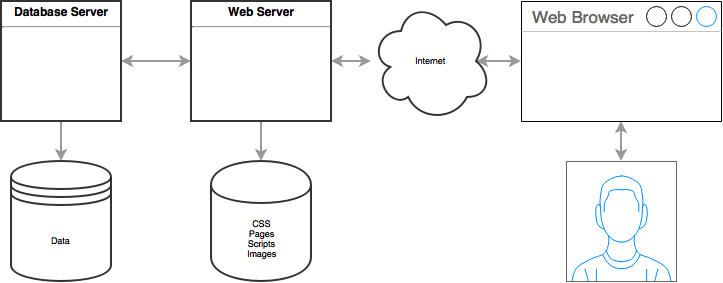
\includegraphics[width=1.0\textwidth]{images/System_Architecture}
	\caption{System Architecture Diagram} \label{fig:System_Architecture}
\end{figure}

The diagram in figure \ref{fig:System_Architecture} depicts the overall system architecture for the proposed solution. The system is broken down into three key components.
\begin{enumerate}
	\item \textbf{Web Browser}: The browser sends a request for a resource of some kind to the web server \cite{AppThena:SystemArchitecture}. The request is generated based on the interaction between the user and the web application, detected by the browser. The browser then displays the response to the request.
	\item \textbf{Web Server}: The web server decides what to do with the request. Static resources such as images, CSS and static web pages are read from disk and returned directly to the browser \cite{AppThena:SystemArchitecture}. Requests for dynamic resources such as as the search pages are processed by requesting the data from the database server.
	\item \textbf{Database Server}: The database server is responsible for hosting a MySQL database which contains all the data. The server then processes queries which either retrieve or update the data.
\end{enumerate}

The web browser presents the user interface to the user based on the response returned. The user directly interacts with the web application by clicking or entering data, which is then detected by the browser and forwarded to the web server. Along with the user interface, the browser is also responsible fir client sided scripts that are executed on the web app. The interaction between the web server and the browser is made possible by the internet. The web server provides a back end for the system and executes a server side scripting language, which in the case of this project is PHP. All the resources for the web application such as pages, stylesheets, scripts, and images are also stored on the web server so they're easily accessible whereas the database and web servers are completely independent. The database server may optionally be stored on the same machine as the web server but this is not necessary. This provides a great level of flexibility for system administrators as one database server can be used to serve several applications, for example a web and mobile application, or numerous database servers for serving one application.

For this project, all servers are installed on a local machine for development purposes but additionally these are also replicated on a VPS for production purposes. The scalability and expansion of this production server is discussed further throughout this report.

\subsection{Database Design}
The successful operation of the system is entirely reliant on the database which stores and provides almost all the content for the system. For a system so dependent on its data, it is crucial that care is taken when developing the database. In order for the system to perform optimally, an efficient database design is required which stores data in a way that minimises redundancy and efficiently utilises space. Various approaches were taken when developing the database to ensure that the data is consistent. As a result of this, data was split up by attributes across a number of tables which relied upon one another through functional dependencies and relationships to provide a collective dataset. These tables are discussed further in section \ref{Section:Database_Tables} followed by an explanation of the normalisation techniques and dependencies introduced in sections \ref{Section:Database_Normalisation} and \ref{Section:Database_Cascading}.

\subsubsection{Tables} \label{Section:Database_Tables}

\begin{figure}[H]
	\centering
	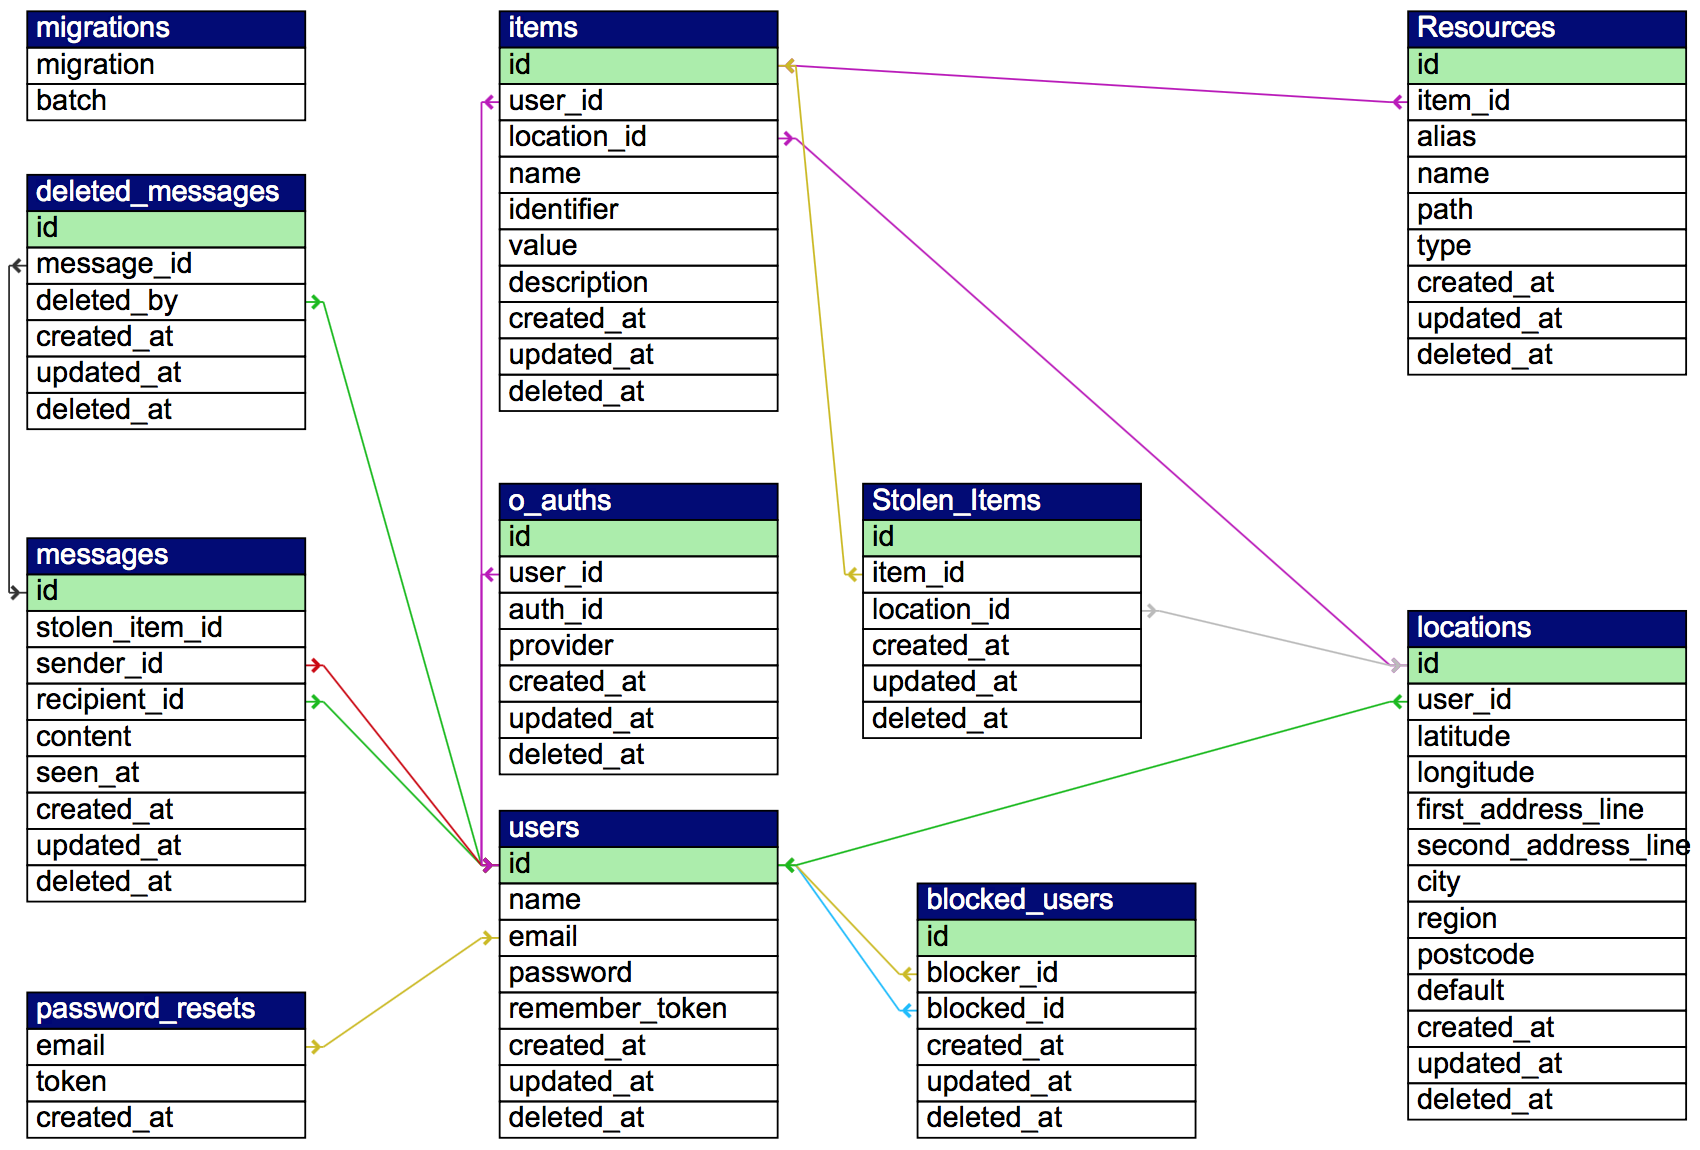
\includegraphics[width=1.0\textwidth]{images/Database/ERD_Plain}
	\caption{Database - Entity Relationship Diagram} \label{fig:ERD}
\end{figure}

The database was designed with modularity in mind. This allowed the database design to be expanded as the system components were built. Each component stores its data in separate tables which rely on the previously implemented components through relational dependencies. The diagram in figure \ref{fig:ERD} shows all the tables in the database and the relationships between these tables. The design of the database and the table choices is discussed further below, categorised by components.

There are some consistent attributes across all the tables shown in the diagram. The id column is used as a primary key to provide each tuple with a unique identifier. This id column is used to manipulate the row based on user input, such as editing and deleting. The last two column store the date on which the tuple was created and deleted. The created at column is never updated and the deleted at column will be null by default, until the user deletes the tuple. This is used for the soft delete feature.

\paragraph{Users} The user component is the core of the system. A significant amount of the functionality provided by the system is reliant on the user system, as can be seen by the dependencies on the user table in figure \ref{fig:ERD}. This means that the user tables are a prerequisite for almost all the components of the system and hence these were the first tables to be designed. The user component was built up of three separate tables. The main table which holds all the user data for authentication and identification purpose is called users. The table has a secondary index, on the email field, in addition to the primary key, which is used for dealing with password reset requests from users. The second table for this component is the password resets table which indexes the rows on the email fields and uses this as a foreign key to associate all requests with a user. The third and final table is the oAuth table used for authenticating users through third-party services such as Facebook and Google. The separate use of an oAuth table for storing tokens allows for the same user to login using various providers rather than creating a new account for each service. These can be seen in figure \ref{fig:ERD_User} below.

\begin{figure}[H]
	\centering
	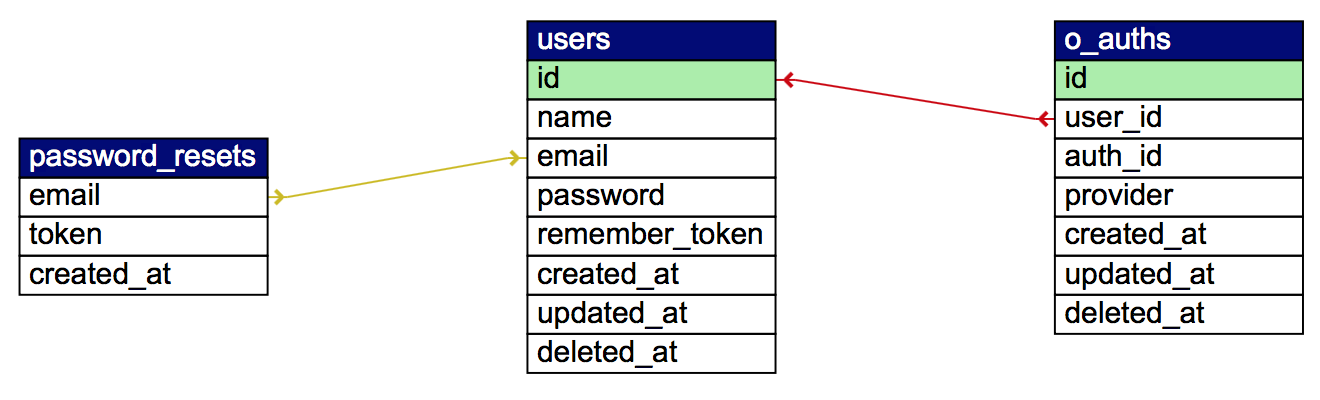
\includegraphics[width=1.0\textwidth]{images/Database/ERD_User}
	\caption{Users - Entity Relationship Diagram} \label{fig:ERD_User}
\end{figure}

\paragraph{Locations} The data for locations was contained solely inside a single table named locations. The table contained a user id column which referenced the id column in the users table as a foreign key. This allowed for locations to be associated with a user, as shown in figure \ref{fig:ERD_Locations}. The initial problem faced by the locations table was that not all addresses have the exact same attributes, e.g. some address may not have a second address line. For this reason a compromise was made to include only attributes that are expected to be available for most addresses. Any additional data could be split across these fields, made possible with the automatic address completion feature that pre-populates these from the post code or coordinates.

\begin{figure}[H]
	\centering
	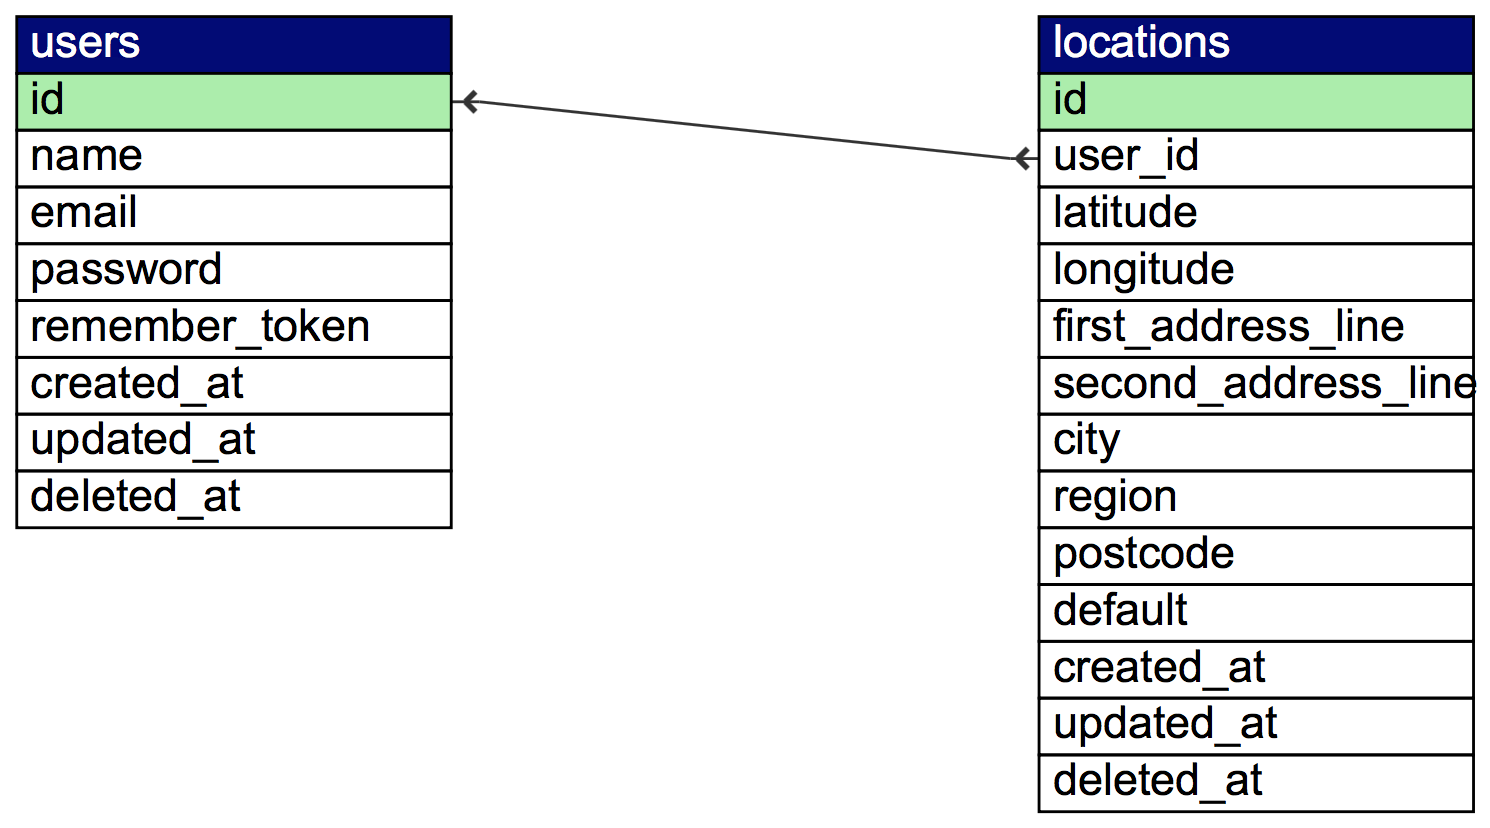
\includegraphics[width=1.0\textwidth]{images/Database/ERD_Locations}
	\caption{Locations - Entity Relationship Diagram} \label{fig:ERD_Locations}
\end{figure}

\paragraph{Items} The design for the tables regarding the items can be thought as two separate designs which are interlinked. An item by default is just for the user who registered it and is associated with the user through a foreign key. This allows for the item to be associated with a location, where it is kept. However, when an item is stolen, it may be stolen from a location other than its registered location and a way to represent this is required. For this reason, a separate table called stolen items was created which stores a tuple that maps an item to a location, allowing for the item to be reported as stolen in a different location. See figure \ref{fig:ERD_Items} for details. 

\begin{figure}[H]
	\centering
	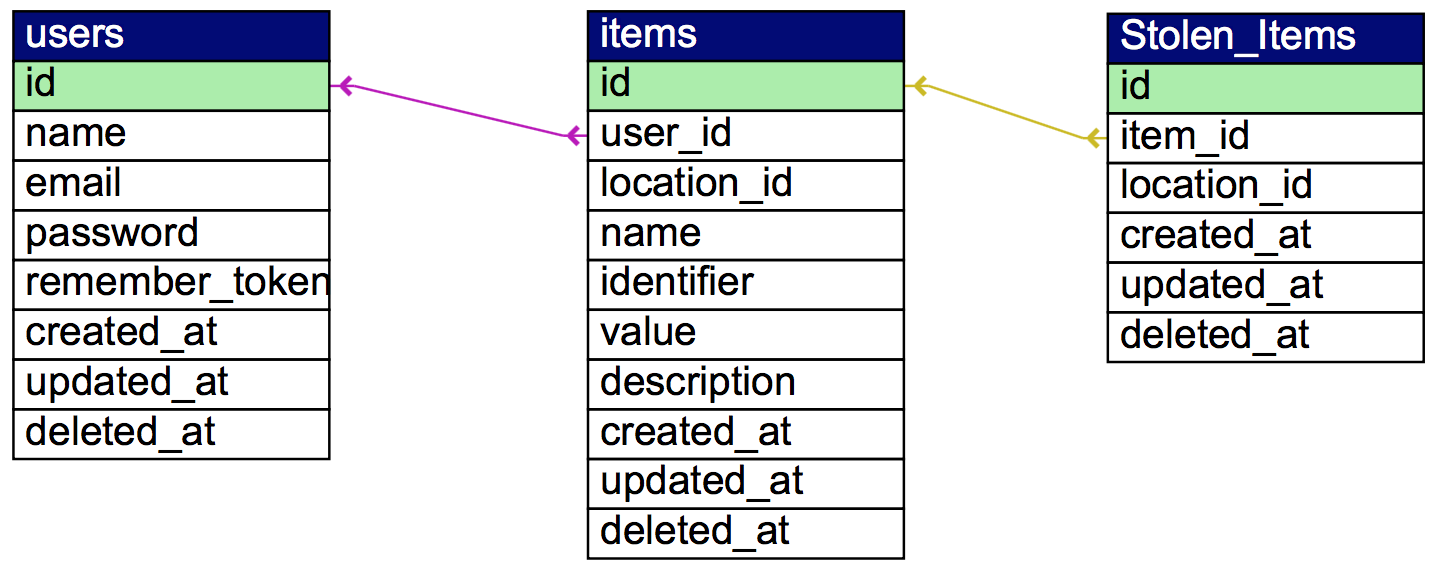
\includegraphics[width=1.0\textwidth]{images/Database/ERD_Items}
	\caption{Items - Entity Relationship Diagram} \label{fig:ERD_Items}
\end{figure}

\paragraph{Resources} The storing of resources relies on a solid implementation of items. A tuple is created for each resource which maps the resource to an item through an item id field. The table does not directly associate the resource with a user but instead the user is indirectly identified through the item. The direct association of a user is unnecessary as it introduces extra columns when the user field is actually never required. 

\begin{figure}[H]
	\centering
	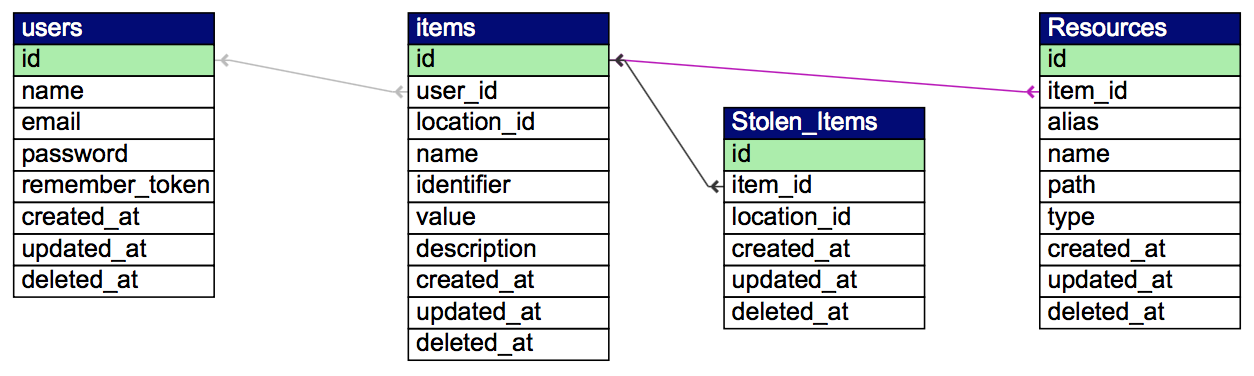
\includegraphics[width=1.0\textwidth]{images/Database/ERD_Resources}
	\caption{Resources - Entity Relationship Diagram} \label{fig:ERD_Resources}
\end{figure}

\paragraph{Messages} The final component to be implemented was the messages component as the tables for this component have a relational dependency on the tables implemented for users, items and the stolen items feature.

\begin{figure}[H]
	\centering
	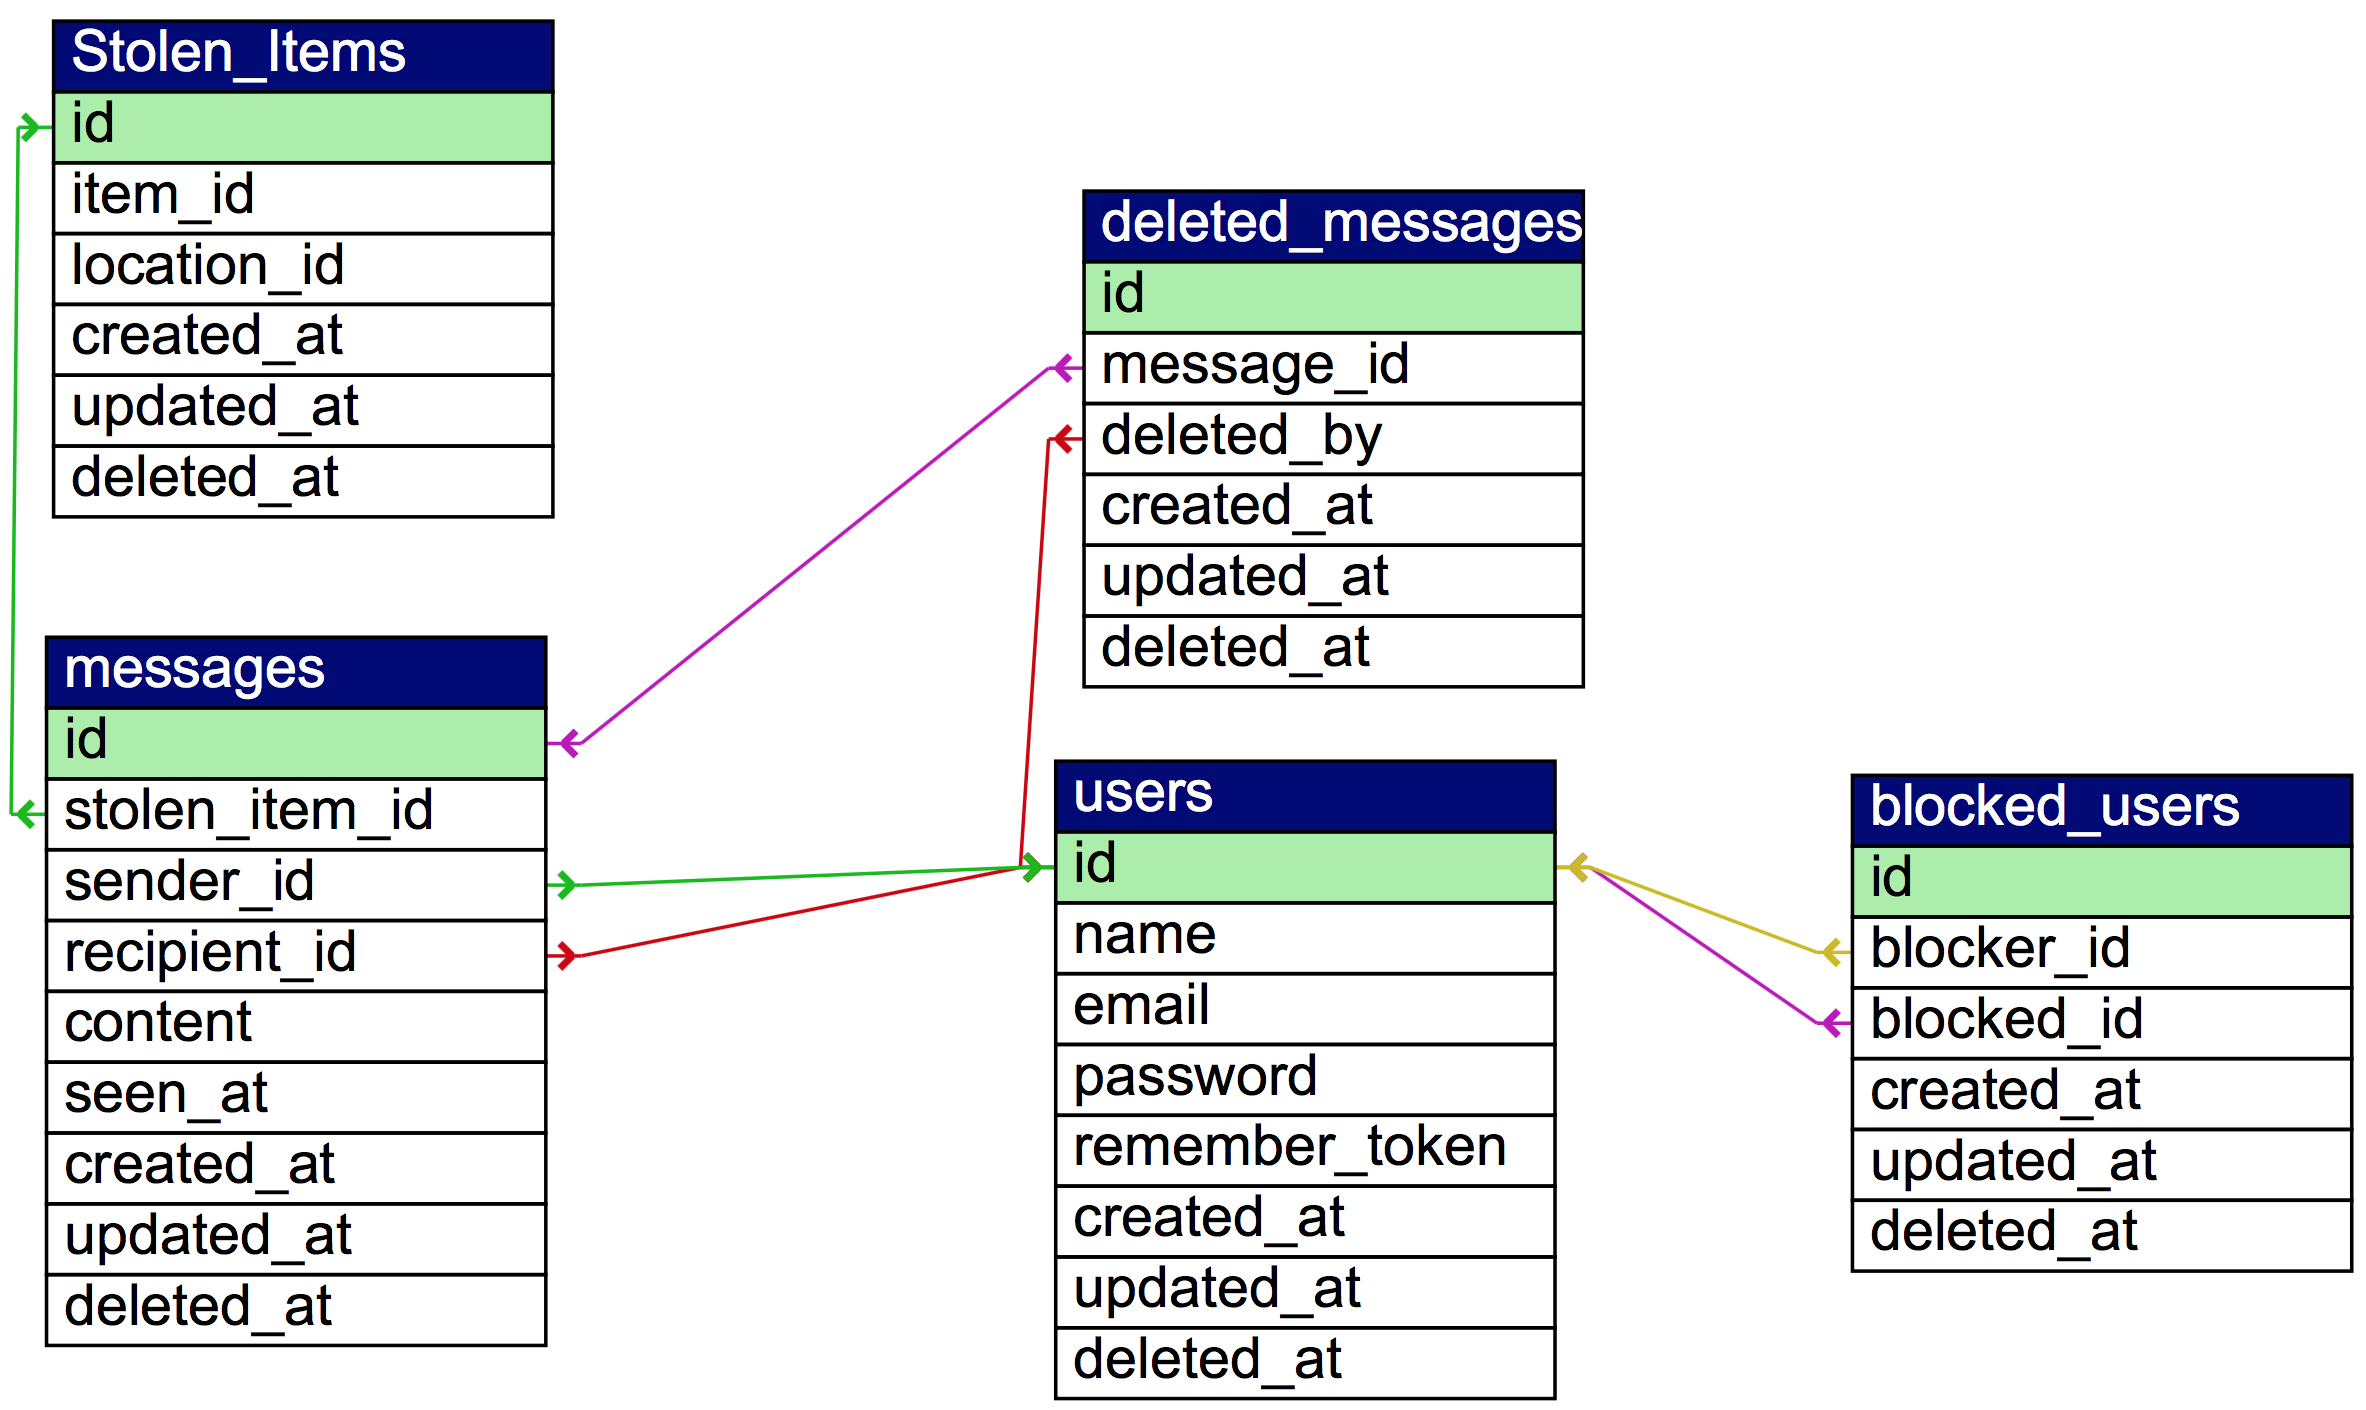
\includegraphics[width=1.0\textwidth]{images/Database/ERD_Messages}
	\caption{Messages - Entity Relationship Diagram} \label{fig:ERD_Messages}
\end{figure}

As visible in the diagram the messages component consists of several tables. Each message is linked to a tuple in the stolen items table instead of the items table. This prevents conversation once the item is recovered. Additionally, each tuple in the messages table is linked to the users table through two separate attributes, the sender id and the recipient id. This allows the users name to be displayed at the top of a conversation for safety reasons. Finally, a link to the deleted messages table exists if a user deletes a message from their inbox. This acts as a soft delete feature for only one participant in the message, soft deleting messages directly in the messages table would remove the message for both the sender and the recipient. The person who deleted the message can be identified via the deleted by column in the deleted messages table which points to a user.\\\\
The tables covered above are the ones that are fundamental for the basic functionality of the system. The thought process stated above was not the initial one but instead a result of several iterations of design and feedback. The commonalities and reasonings behind the design are discussed further in the following sections.

\subsubsection{Normalisation and Redundancy} \label{Section:Database_Normalisation}
''Normalisation is the process of efficiently organising data in a database. There are two goals of the normalisation process: eliminating redundant data and ensuring data dependencies make sense.'' \cite{Databases:NormalisationBasics}. There are various normal forms that a database can be normalised to, starting at first normal form. Each time a database is normalised further it usually results in data being split up into more table and more dependencies being created. The database for the system was normalised to third normal form as this removed all redundant data from the tables whilst providing dependencies that made sense.

\begin{figure}[H]
	\centering
	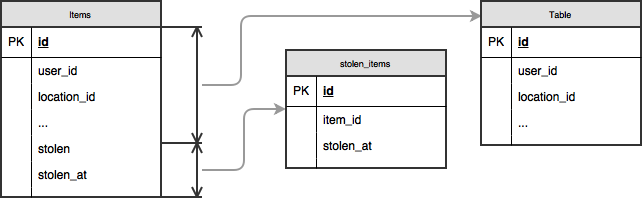
\includegraphics[width=1.0\textwidth]{images/Database/3NF_Items}
	\caption{Items Table - Original vs Third Normal Form} \label{fig:3NF_Items}
\end{figure}

Third normal form expects that the requirements for all the previous normal forms are met and any columns that are not dependent upon the primary key should be removed \cite{Databases:NormalisationBasics}. The items and stolen items table are a result of the third normal form being applied to the items table. Initially, the items table contained a column called stolen which held a boolean true or false and a column called stolen at which held the id of the location where the item was stolen. Once normalised, the attributes are moved into a separate table as shows in figure \ref{fig:3NF_Items}.

\subsubsection{Foreign Key Constraints} \label{Section:Database_Cascading}
In a large normalised database with several tables, it is often the case that information in one table relates to information in another table. SQL dependencies are the by-name references, that are used in SQL expressions, that make one entity reliant on another entity \cite{Microsoft:Dependencies}. An entity being referenced by another entity is known as a referenced entity whereas an entity referencing another entity is known as a referencing entity. There are two different types of dependencies that can be introduced into a database.
\begin{itemize}
	\item \textbf{Schema-bound dependency}: A schema-bound dependency is a relationship between two entities that prevents the referenced entity from being dropped or modified as long as the referencing entity exists \cite{Microsoft:Dependencies}.
	\item \textbf{Non-schema-bound dependency}: A non-schema-bound dependency is a relationship between two entities that does not prevent the referenced entity from being dropped or modified \cite{Microsoft:Dependencies}.
\end{itemize}
Dependencies can be defined in an SQL schema when creating tables by using the references keyword which links an attribute in one entity to an attribute in another. This prevents data being inserted into the referencing entity if the exact value for the attribute does not exist in the referenced entity. This feature is known as referential integrity and prevents redundant data building up in the database. Additionally the administrator can specify the effects of a change in the referenced entity.

In the database design, either directly or indirectly, dependencies were used to link all the entities to one another. This can be seen by the links between tables in figure \ref{fig:ERD}. The relationships among these entities vary between a one-to-one relationship and a one-to-many relationship depending on the type of data being stored. For example, a user can have many locations so a one-to-many relationships exists between the users and locations table. Majority of the foreign key constraints used in the database were setup with cascade delete and cascade update. This means that if a row in the referenced entity is removed or updated then any rows in the referencing entity which correspond to it are also updated or deleted \cite{TechOnTheNet:Cascading}. Some of the constraints followed the schema-bound dependencies by using the restrict keyword which prevents changes in the referenced entity if corresponding rows exist in the referencing entity. The use of all these techniques ensures that data is always kept consistent and no redundant data is introduced into the system.

\subsubsection{Security}
Security is of the upmost importance when it comes to a database which contains sensitive or personal information about individuals. For this reason, several measures should be taken into consideration to protect the database and the data in it from unauthorised access. The security threats and approaches taken to protect against them are discussed below.

\paragraph{Access}
The first step to protecting the data is controlling who has access to the database and who is authorised to do what. This was achieved by creating separate SQL user accounts with different privileges. The database was then protected using a password to prevent any unauthorised access and only authorised users with a username and password would be able to access the database. Furthermore, each user was restricted so that the database would accept connections from the user if they were from a specified IP address. This meant that database connections could be restricted to just the web server and any users attempting to connect to the database from other machines would be denied access. When connecting to the database through PHP, root account was used for development purposes to prevent any restrictions but a separate account was used for production which was unable to modify the schema but could still query or modify the data.

\paragraph{SQL Injection}
,,SQL injection is a technique where malicious users can inject SQL commands into an SQL statement, via web page input'' \cite{W3Schools:SQL_Injection}. According to a report on 5,500 companies and 15,000 websites, almost half of these were vulnerable to serious security threats by XSS or SQL injection \cite{FirstPost:Vulnerabilities}. SQL injection can lead to all the data held in a database being made available. This is a serious threat as some of the data can be used to identify individuals and measures should be introduced to protect against this. One way to prevent SQL injection is by escaping all user input to prevent users from executing malicious queries. This is not a full fix for the issue as users can still enter data that can cause the system to malfunction. The alternative fix for this was using prepared queries which executes the query with placeholders and then binds the values later to retrieve the records. This method escapes SQL injection and prevents any unauthorised interaction with the database.


\subsection{User Interface Design}
The user interface is perhaps one of the most important aspects of the whole system. The system needs to be able to engage the audience from the moment they land on the homepage and encourage the users to explore further by providing an easy to use and intuitive UI. This can be achieved by following standards defined by several committees and adhering to good practices. In addition to the engagement the system also needs to be usable whilst being simple and intuitive. Responsive design is also crucial to provide access to the system across a range of devices. The designs were initially made as quick mockups using bootstrap without much styling but screenshots of the end products are included for reference.

\subsubsection{Usability}
In order for a system to be successful and adopted by its target audience, it must be easily usable. For decades, research has been conducted around the usability of systems and peoples reactions to it. The field known as human–computer interaction (HCI) researches the design and use of computer technology, focusing on the interfaces between people (users) and computers \cite{Wiki:HCI}.

Everyday systems are being redesigned due to human need for simplicity. Web applications have progressed a lot since their earlier days when the technology was limited. Today such a large range of web development technologies exist which allow websites to be created with ease and also make usability a worry of the past. Figure \ref{fig:Facebook_Changes} shows a comparison between a 2004 and 2016 version of the most popular social platform, Facebook. The comparison depicts the change that has been brought about in just over a decade.

\begin{figure}[H]
	\centering
	\begin{subfigure}[t]{0.45\textwidth}
		\centering
		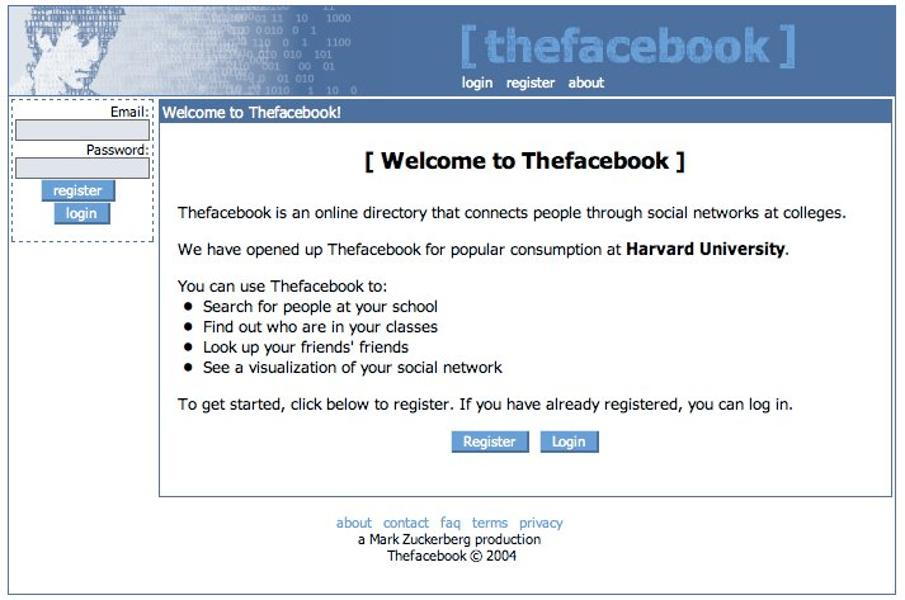
\includegraphics[width=1.0\textwidth]{images/Facebook_2004}
		\caption{Facebook in 2004}\label{fig:Facebook_2004}		
	\end{subfigure}
	\quad
	\begin{subfigure}[t]{0.45\textwidth}
		\centering
		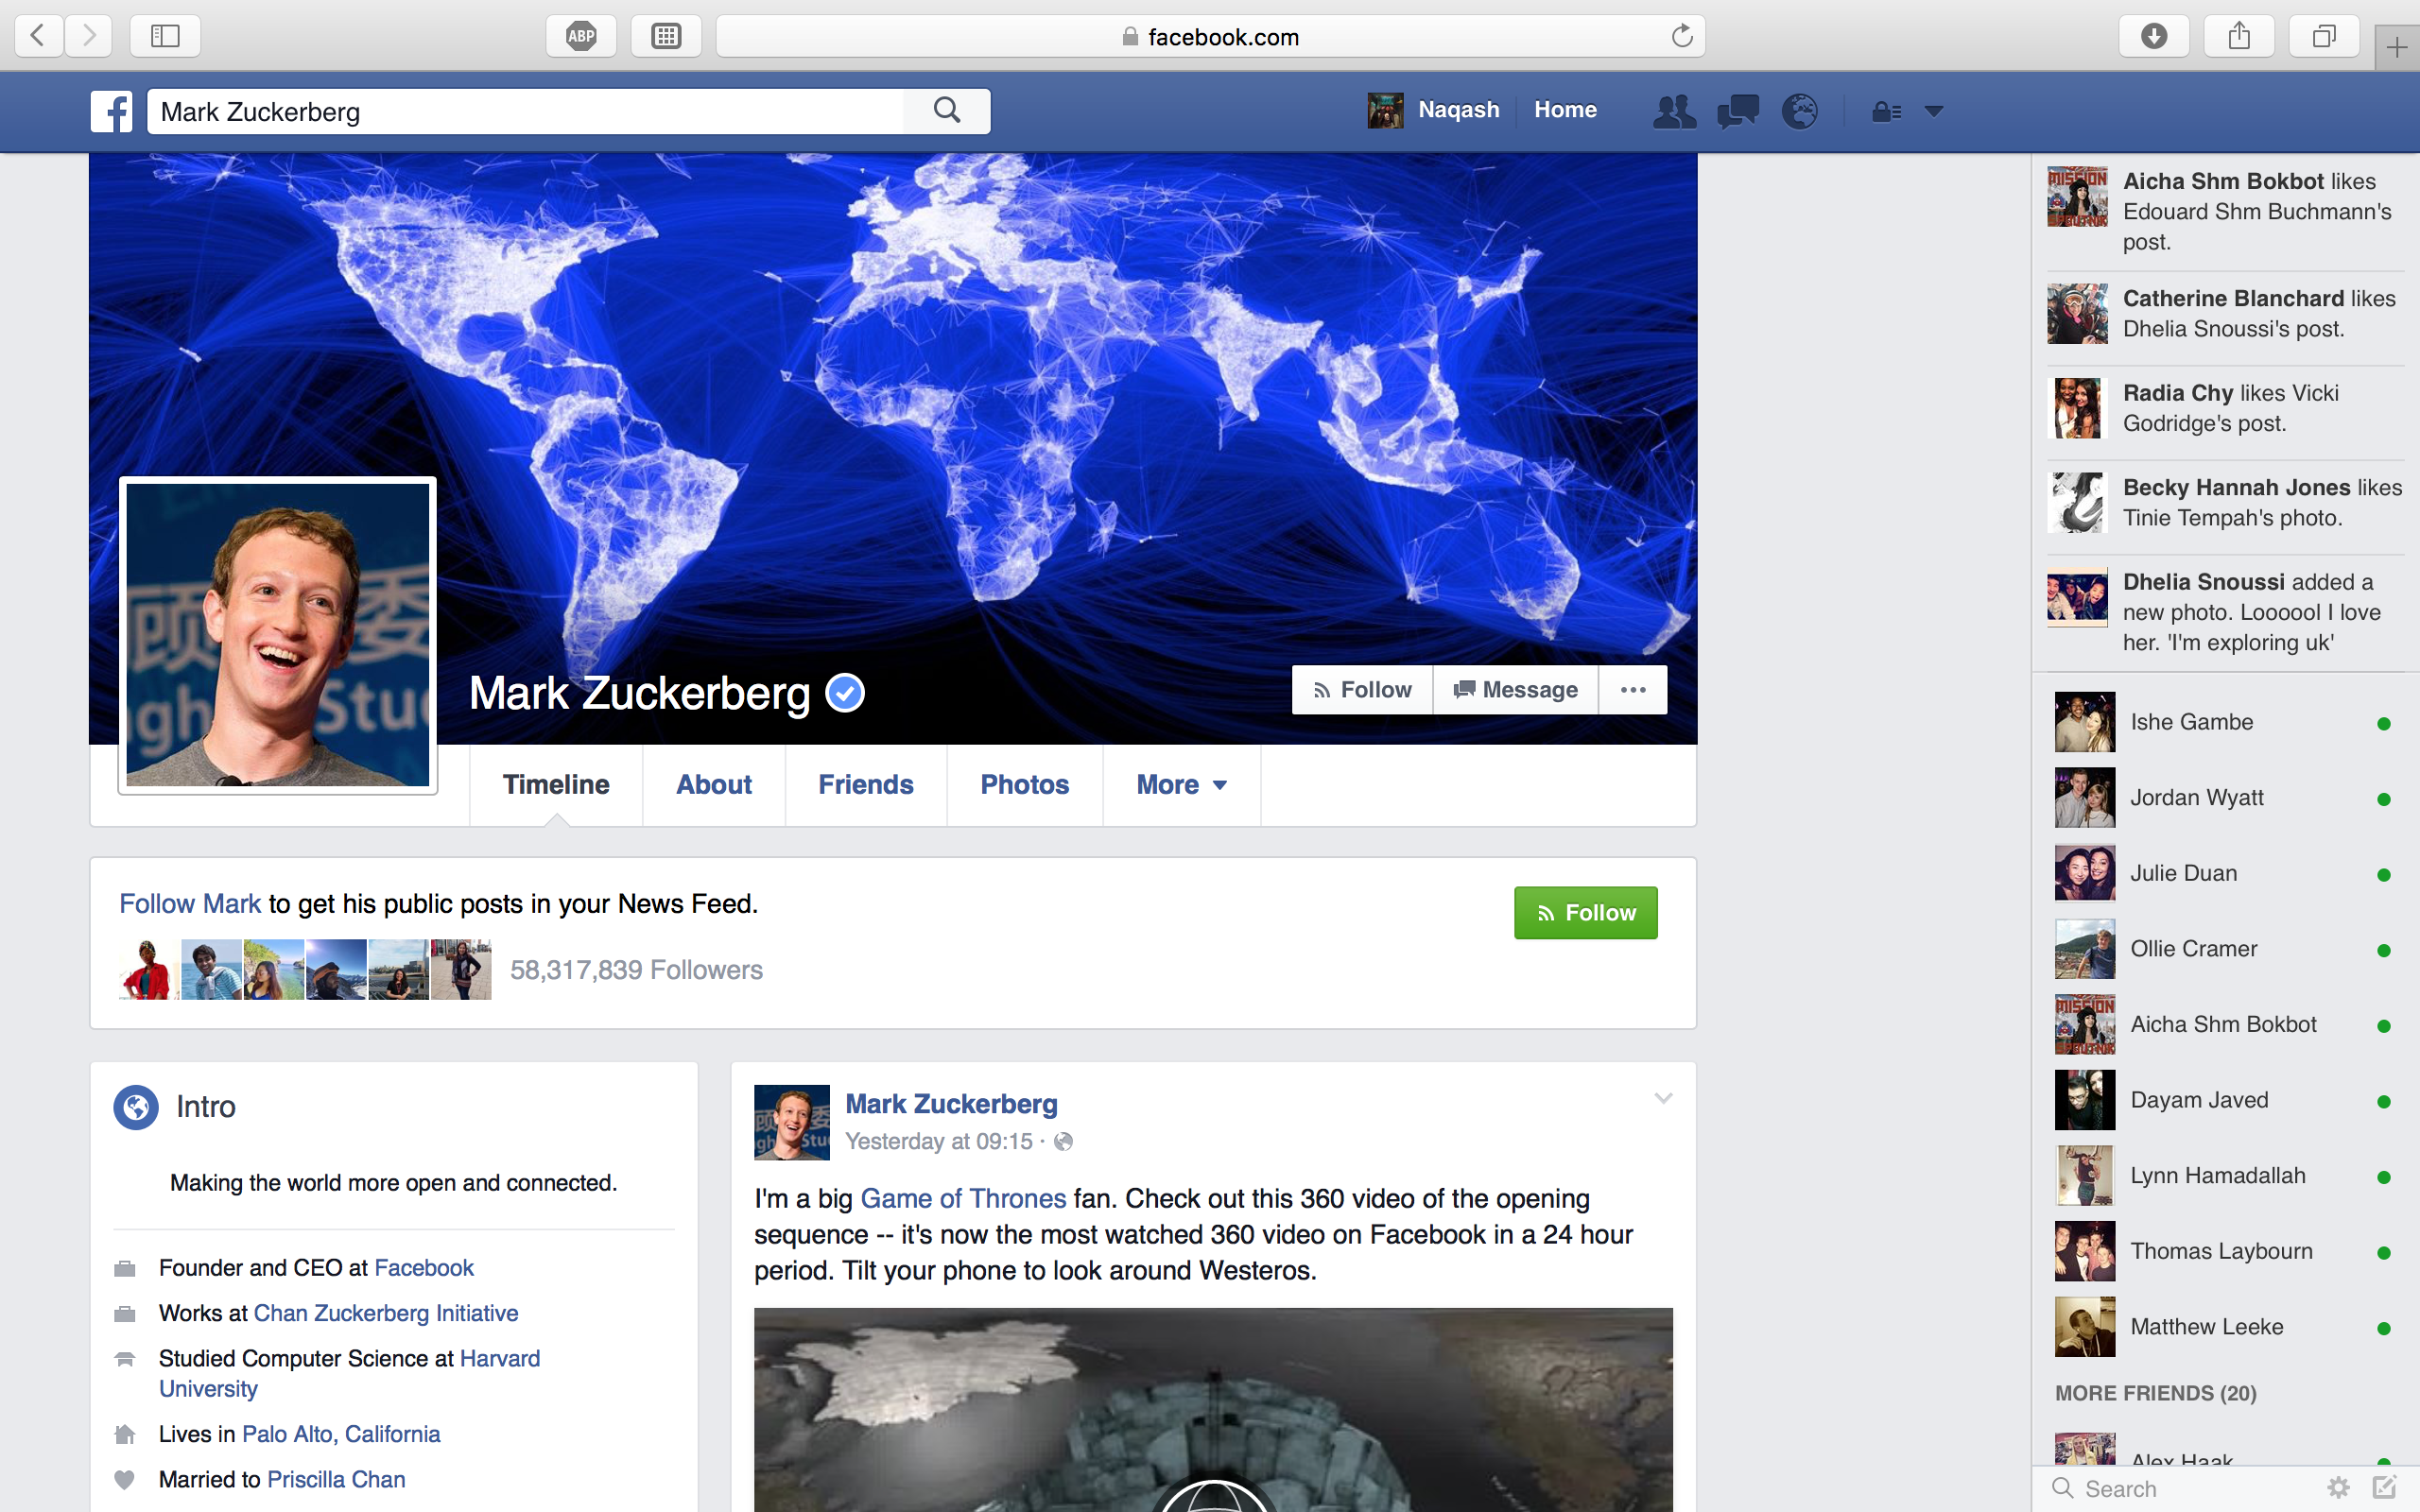
\includegraphics[width=1.0\textwidth]{images/Facebook_2016}
		\caption{Facebook in 2016}\label{fig:Facebook_2016}
	\end{subfigure}
	\caption{Facebook in 2004 vs 2016}\label{fig:Facebook_Changes}
\end{figure}

\paragraph{Intuitive Design} Intuitive designs not only make web applications more usable but they also reduce the amount of time it takes to accomplish tasks using the system. Using the example of Facebook, initially users would enter a search query which would redirect them to the search page but now it is possible to simplify features like search using a simple AJAX dropdown which live updates whilst searching. This is just one example of how intuitive systems can be built and usability can be improved. Another example of intuitive design is the use of images and icons, such as the bell icon for notifications and the magnifying glass icon for search, that have a clear meaning. This is demonstrated in figure \ref{fig:Consistent_Navigation} where the icons used in both navigations are either the exact same or very similar.

\paragraph{Flat Design} Another change that has been brought about to improve the usability of systems is the use of flat colours for design over gradients and textures. In the past, gradients were commonly used across web applications to make the website stand out but they often make the page seem crowded. In recent years many systems, lead by Microsoft, have adopted a flat design approach in which simple and plain colours are used for design to make the page appear cleaner. This makes navigating the page easier and allows more content to be added to the page without making it seem cluttered. An example of this is shown in figure \ref{fig:Twitter_Changes} where the initial twitter design which uses heavy shadows and gradients has been transformed into a clean user interface which uses just plain colours such as white and black along with orange.

\begin{figure}[H]
	\centering
	\begin{subfigure}[t]{0.45\textwidth}
		\centering
		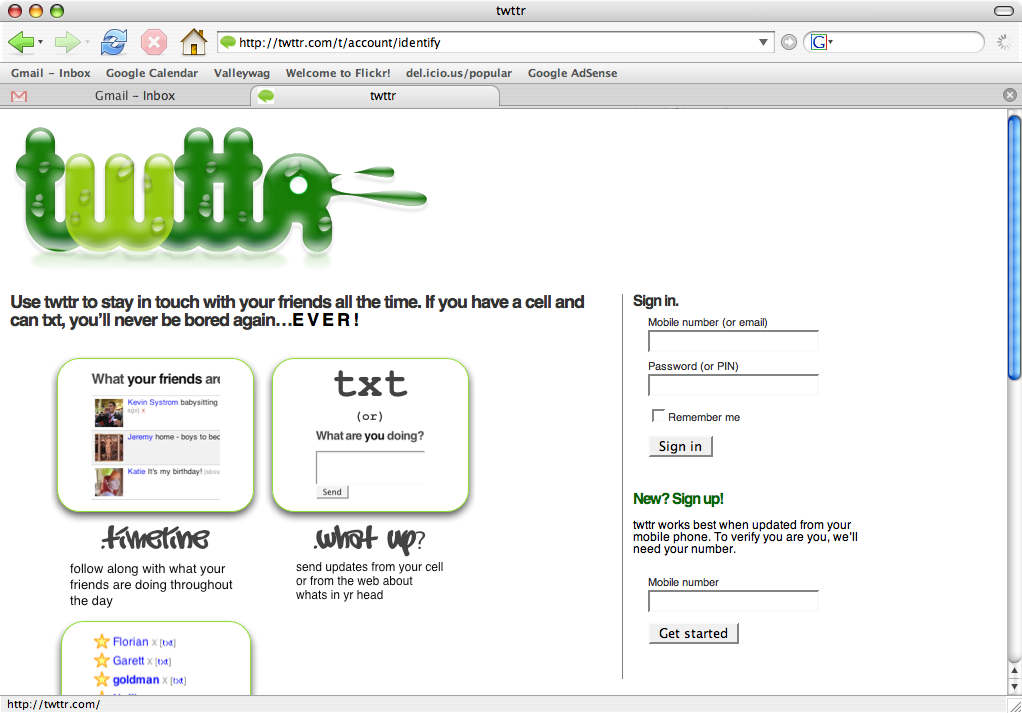
\includegraphics[width=1.0\textwidth]{images/Twitter_Old}
		\caption{Twitter - First Release}\label{fig:Twitter_Old}		
	\end{subfigure}
	\quad
	\begin{subfigure}[t]{0.45\textwidth}
		\centering
		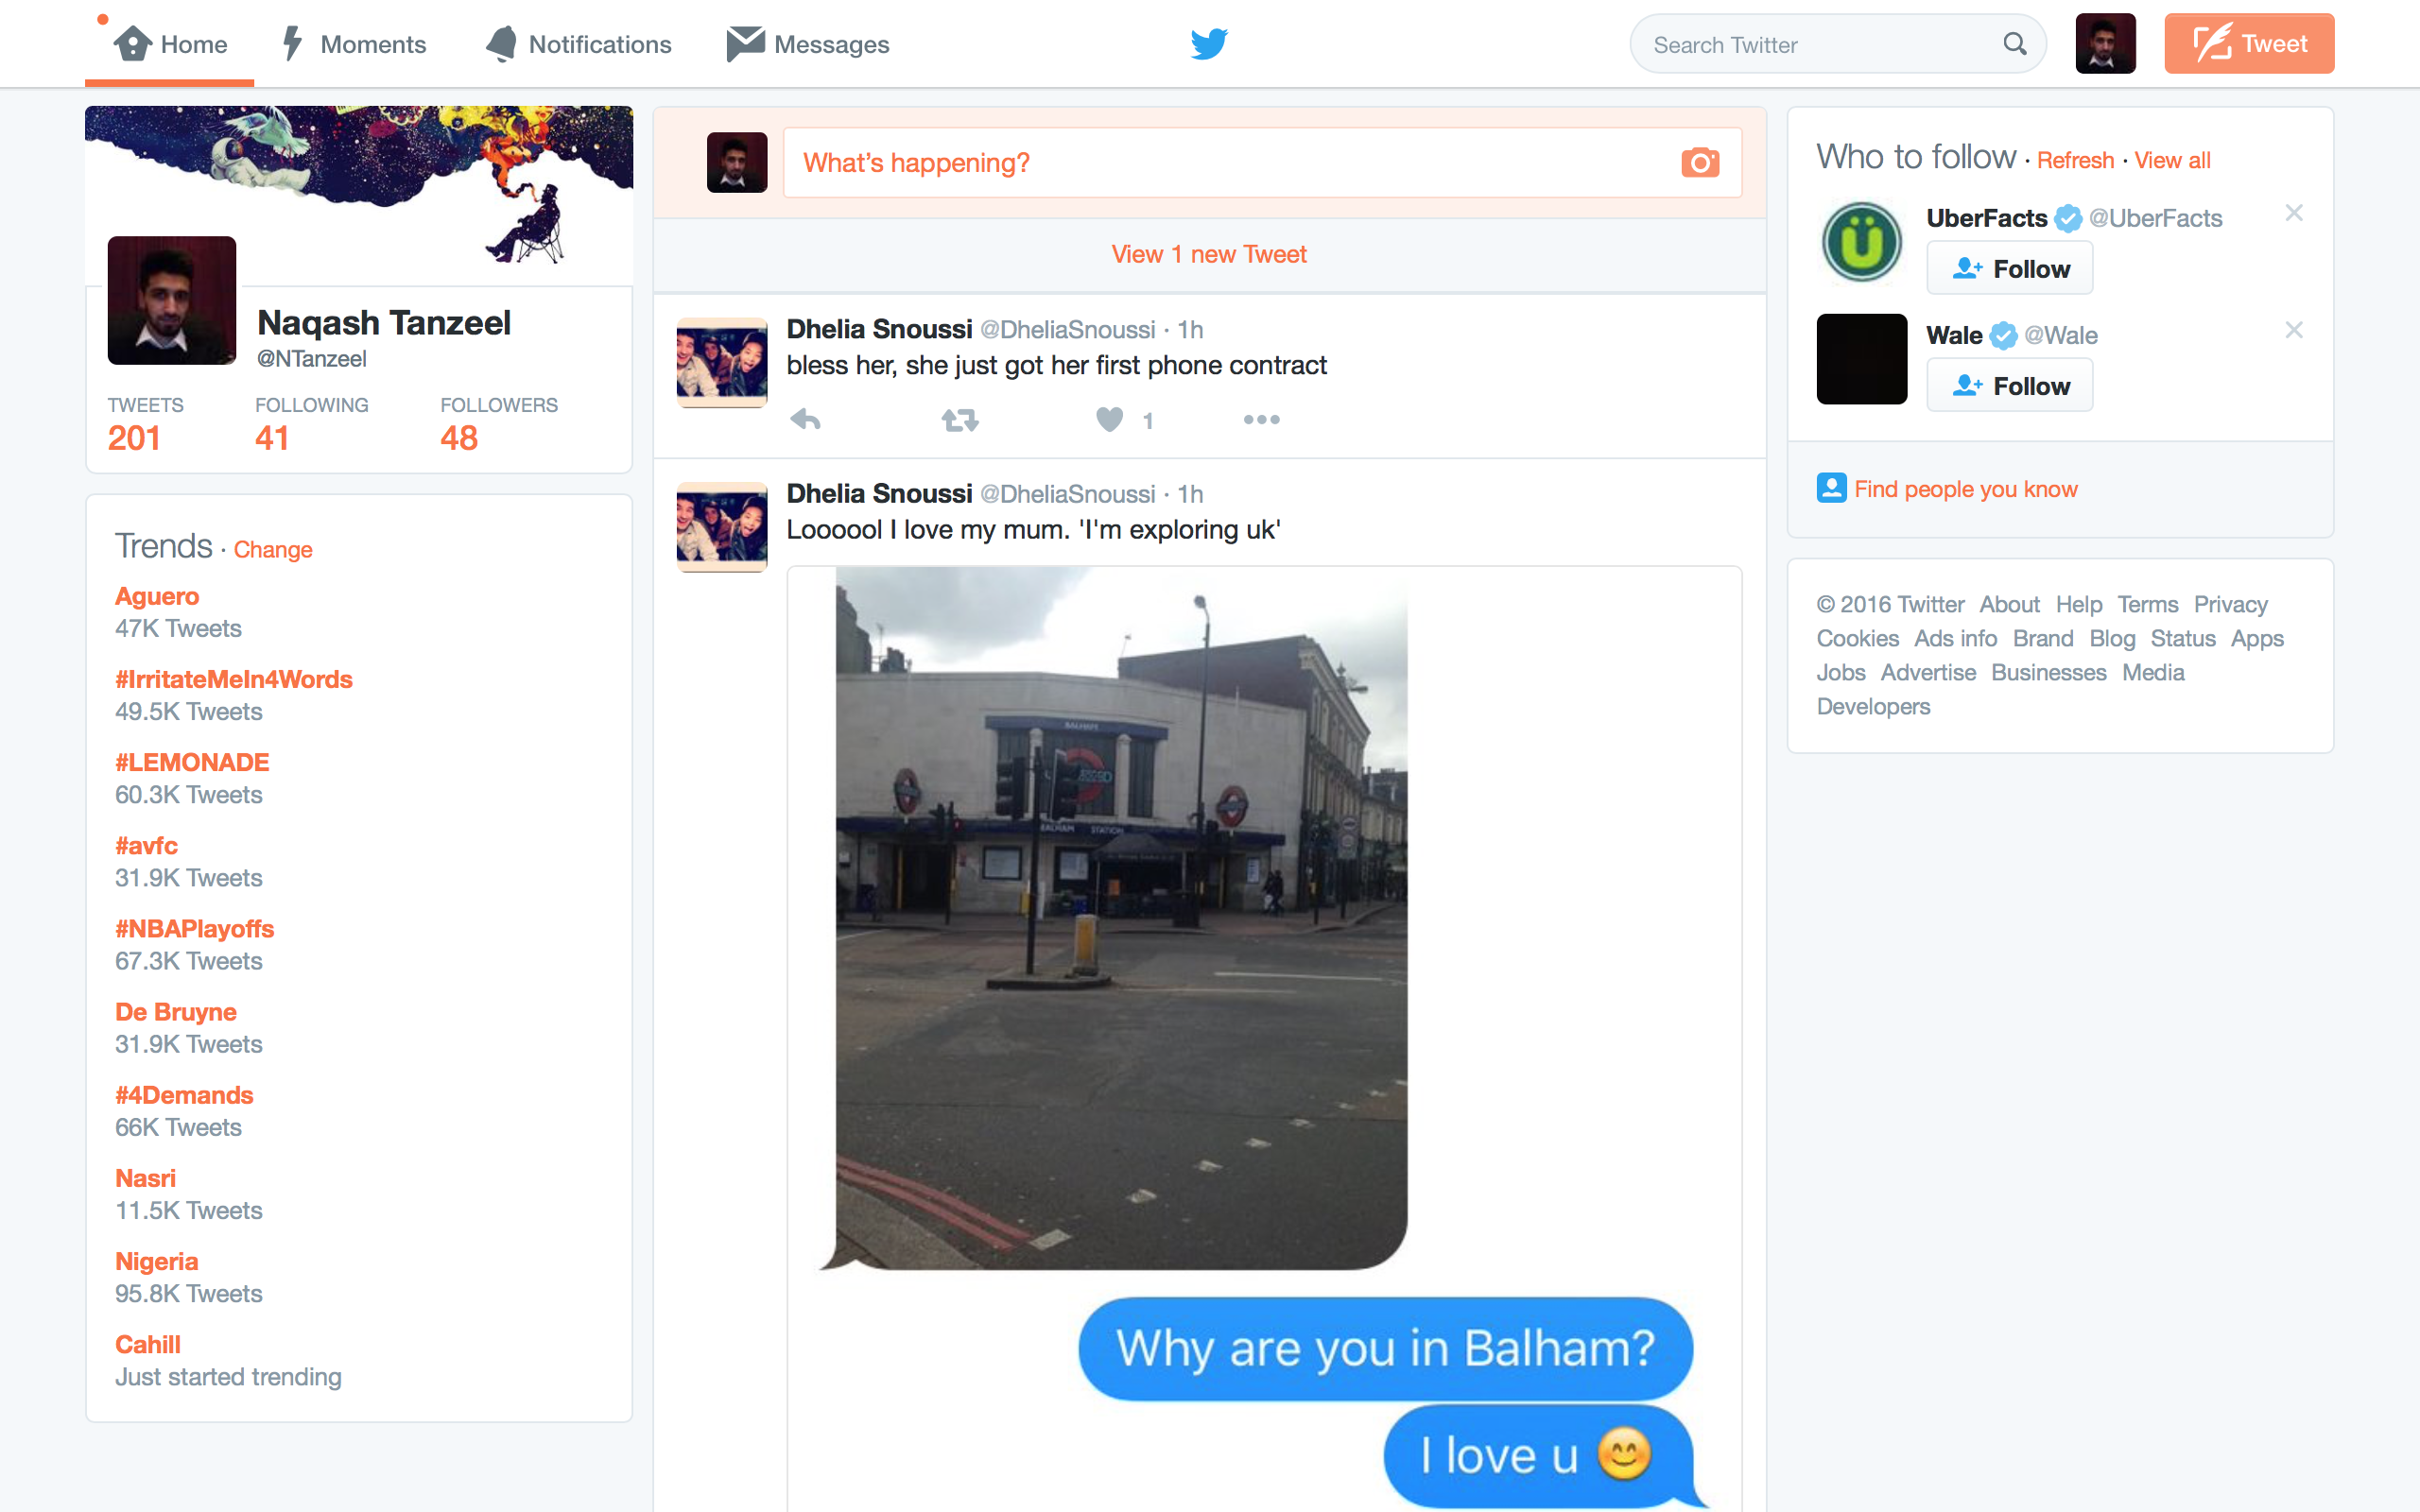
\includegraphics[width=1.0\textwidth]{images/Twitter_Flat}
		\caption{Twitter - 2016}\label{fig:Twitter_Flat}
	\end{subfigure}
	\caption{Twitter Original vs 2015}\label{fig:Twitter_Changes}
\end{figure}

\subsubsection{Consistency}
Consistency plays a key role when it comes to assessing how usable a system is. It has been found that part of usability is consistency across a system. The use of consistent features across pages simplifies the experience for the user as they will already know how to interact with certain parts of the page. An example is the placement of the navigation near the top of the page or a sidebar which are consistent across almost all websites, as shown in figure\ref{fig:Consistent_Navigation} for Facebook and Twitter. This reduces the amount of confusion the user faces whilst trying to work their way around the website.

\begin{figure}[H]
	\centering
	\begin{subfigure}[t]{1\textwidth}
		\centering
		
\includegraphics[width=1.0\textwidth]{images/Facebook_Nav}
		\caption{Facebook Global Navigation Bar}\label{fig:Facebook_Nav}		
	\end{subfigure}
	\quad
	\begin{subfigure}[t]{1\textwidth}
		\centering
		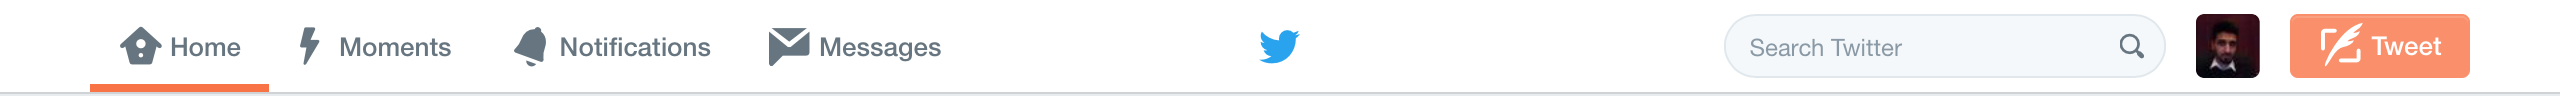
\includegraphics[width=1.0\textwidth]{images/Twitter_Nav}
		\caption{Twitter Global Navigation Bar}\label{fig:Twitter_Nav}
	\end{subfigure}
	\caption{Consistent Navigation Bar Placement}\label{fig:Consistent_Navigation}
\end{figure}

\paragraph{Navigation} During the design this technique was adopted and on all the public pages the design was kept consistent by providing a navigation bar at the top of every page. Intuitive icon were used in the navigation for each of the links to make it clear to the user what each function will do. These were adopted from the examples shows in figure \ref{fig:Consistent_Navigation} and can be seen in figure \ref{fig:Frisk_Nav}. In addition to this, the colours and spacing of content was also kept consistent, the implementation details of which are discussed further in section \ref{Section:Implementation}. On the private user pages accessible through the dashboard a consistent navigation was provided through a sidebar. A header template was also provided which was populated depending on each page but the design was kept the same regardless of page.

\begin{figure}[H]
	\centering
	
\includegraphics[width=1.0\textwidth]{images/Frisk/Frisk_Nav}
	\caption{Frisk - Navigation Bar} \label{fig:Frisk_Nav}
\end{figure}

\subsubsection{Initial Designs}
Initially it was decided that the web app design would be kept consistent across all pages. This meant including the same navigation bar and theme on all pages and any pages which required authentication would be placed in a menu under the users name. Alternatively some of the the authentication links could also be included in the navigation itself, as with the other links on the right. This would allow for a pleasant user experience and familiarity across all pages. In addition, this would mean that only one master layout would have to be designed and the rest of the pages would be able to extend this layout.

After the requirements from the specification were adapted during the development of features for an authenticated user an alternative approach was adopted. The expansion in requirements meant that a lot more functionality was required for authenticated users and the single top navigation approach would not be sufficient. As a result the system was designed as two separate systems with entirely different designs. The simple clean design was used for all the front end public pages that were available to all users, whether registered or not. Important links such as messages were still kept in the navigation bar across all pages if the user was logged in and a link to the dashboard replaced the sub-links in the user dropdown.

A second design was used in the dashboard and all the links were moved from the user dropdown to the dashboard sidebar. This allowed for a main navigation in the sidebar which allowed users to navigate key components such as items and location but then sub components such as create and delete links were incorporated outside of the sidebar. The use of this template allowed for more space to be utilised vertically without having to remove the navigation bar if the content was overflowing and the user was forced to scroll. The use of a sidebar also made the dashboard much more user friendly on mobile devices.

\subsection{Page Designs}
Pages refers to the public parts of the web application which can be accessed without authenticating in contrast to the dashboard which is only available to authenticated users. These include the homepage, search page, and the explore page. The template for pages will be kept relatively simple with a single navigation bar at the top and a container which will hold the content per page. The design and the reasons behind the choices made are discussed in the following subsections.

\subsubsection{Homepage}
The homepage for the website was kept simple in design. The same navigation as all other public pages was used to reduce confusion and increase familiarity for the user. The page consisted of a map and just a simple search field. The markers on the map highlight all the burglaries that have happened in the users postal area. The purpose of the map was to highlight the crime in the users area which would hopefully encourage them to signup for the system in order to protect their valuables.

\begin{figure}[H]
	\centering
	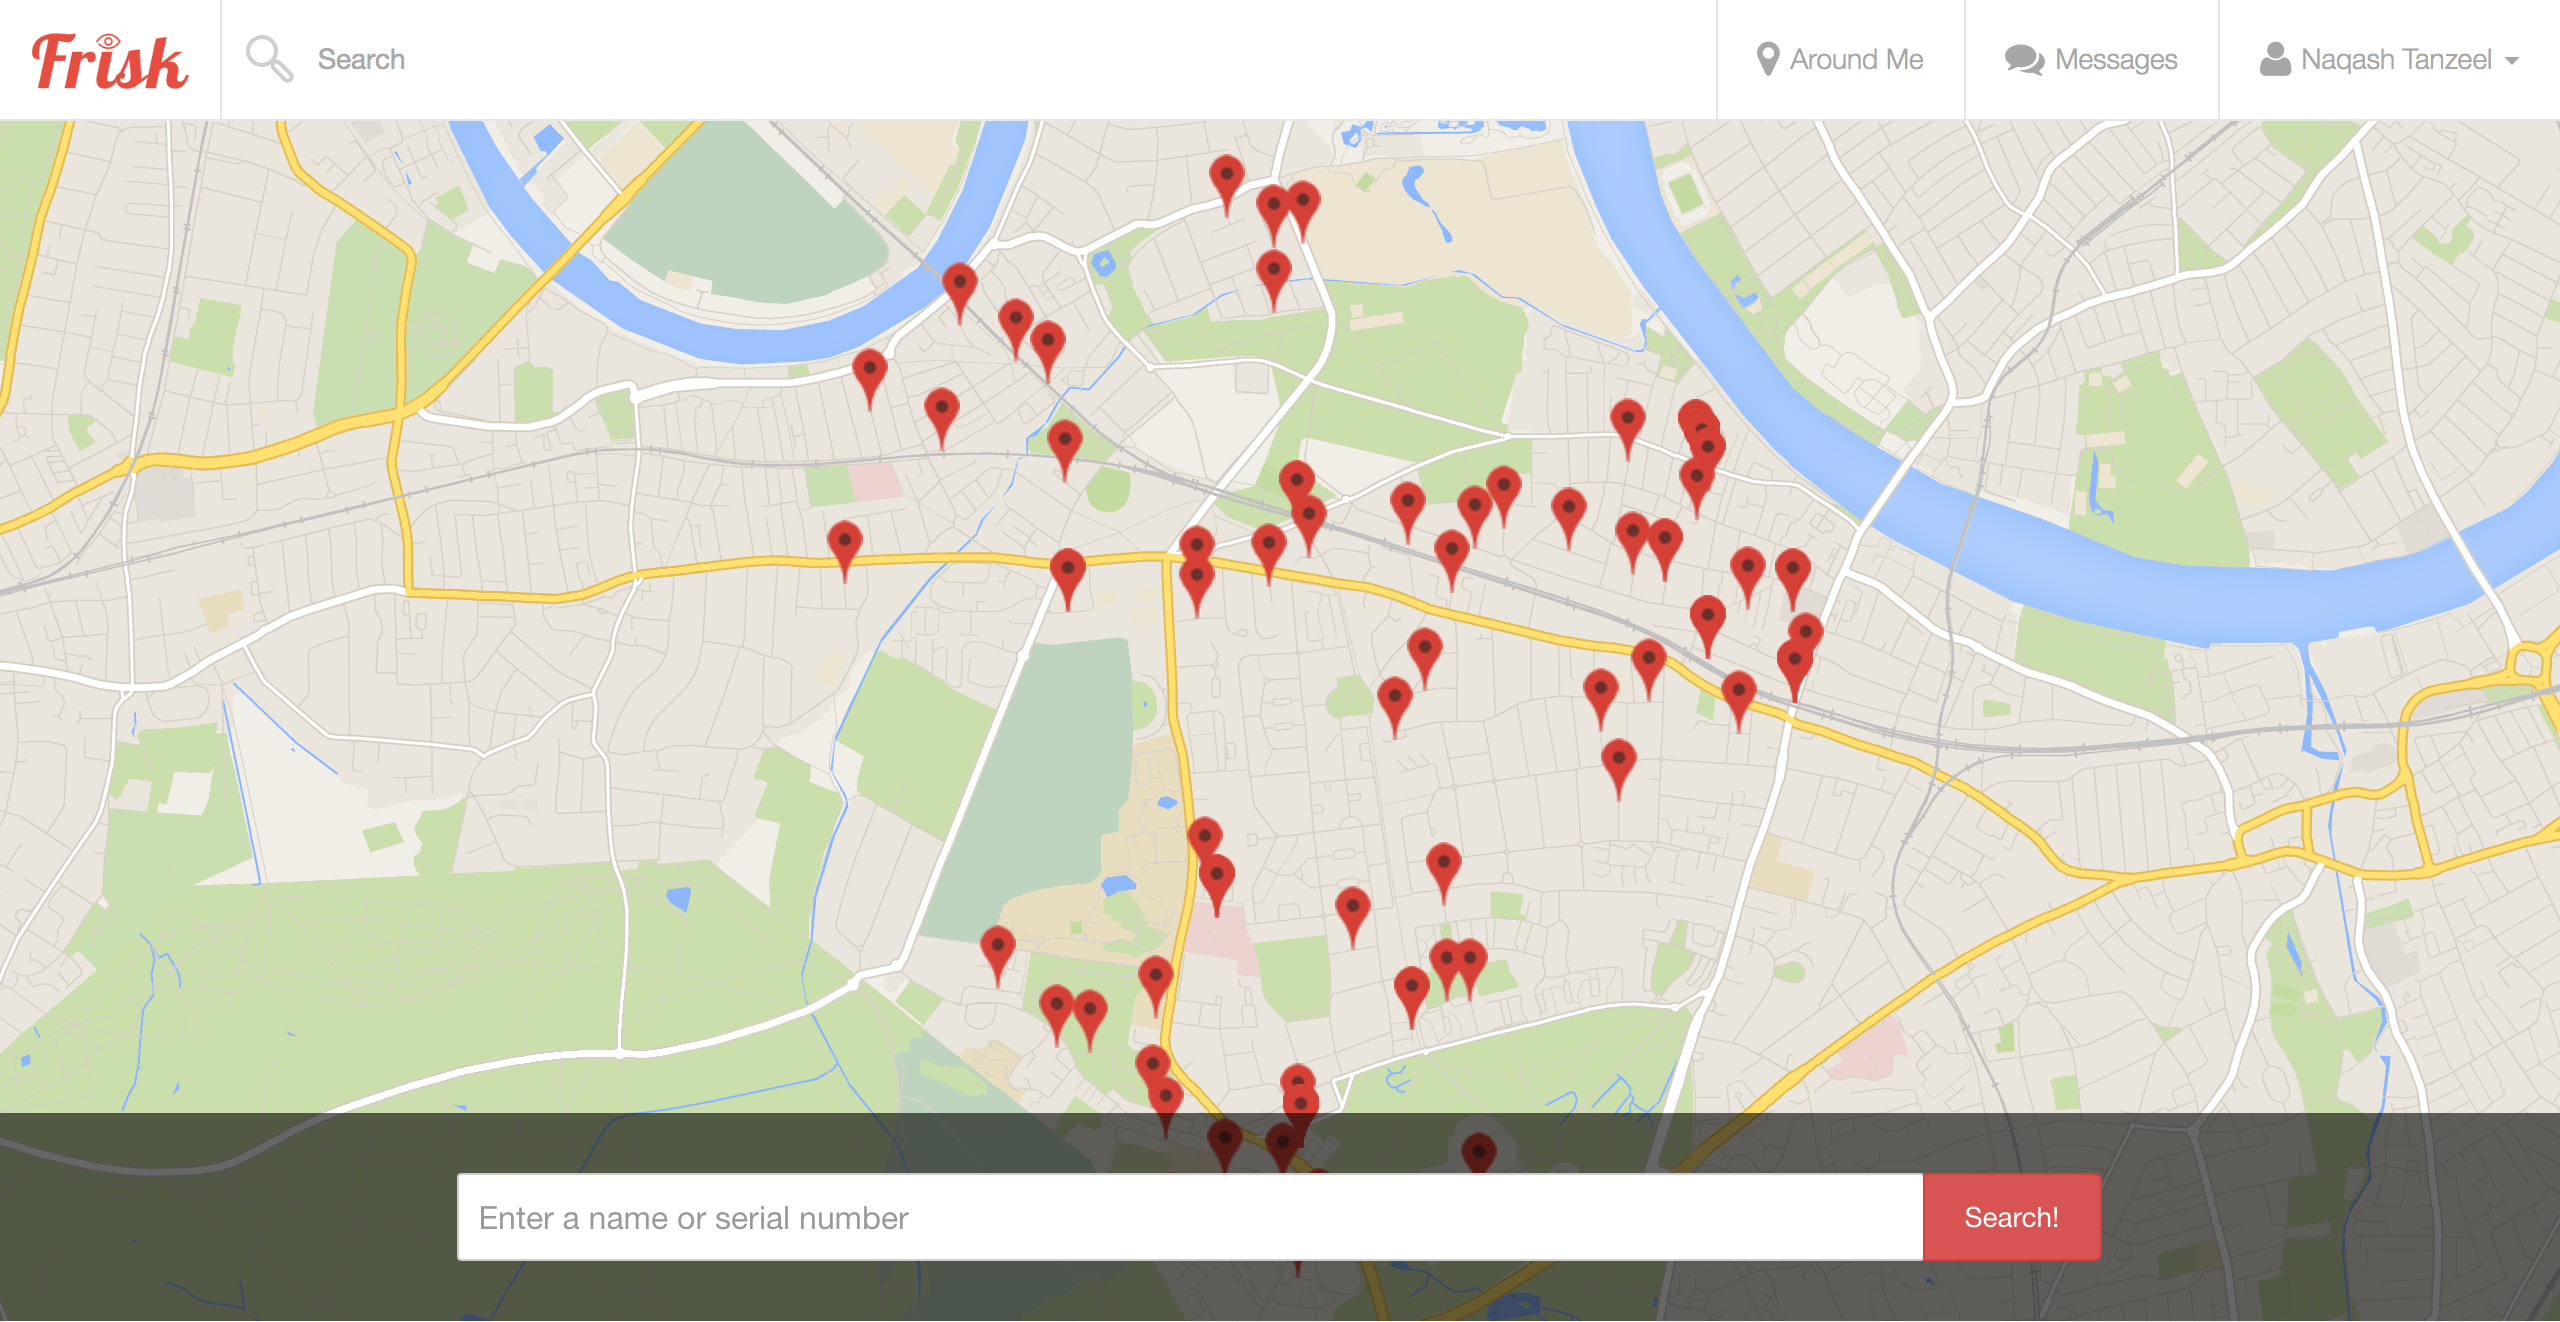
\includegraphics[width=1.0\textwidth]{images/Frisk/Page_Home}
	\caption{Frisk - Homepage} \label{fig:Page_Home}
\end{figure}

The design shown in figure \ref{fig:Page_Home} is just a mockup that was created by prototyping through web development tools and has minimal information. The the actual implementation of the homepage should provide more functionality but it is not a necessity. This is because the homepage is designed as a welcome page and does not actually need to provide any functionality. One of the initial purposes of the homepage was to accommodate the search feature, as shown in figure \ref{fig:Page_Home}, but this was later also included in the navigation bar.

\subsubsection{Search}

\begin{figure}[H]
	\centering
	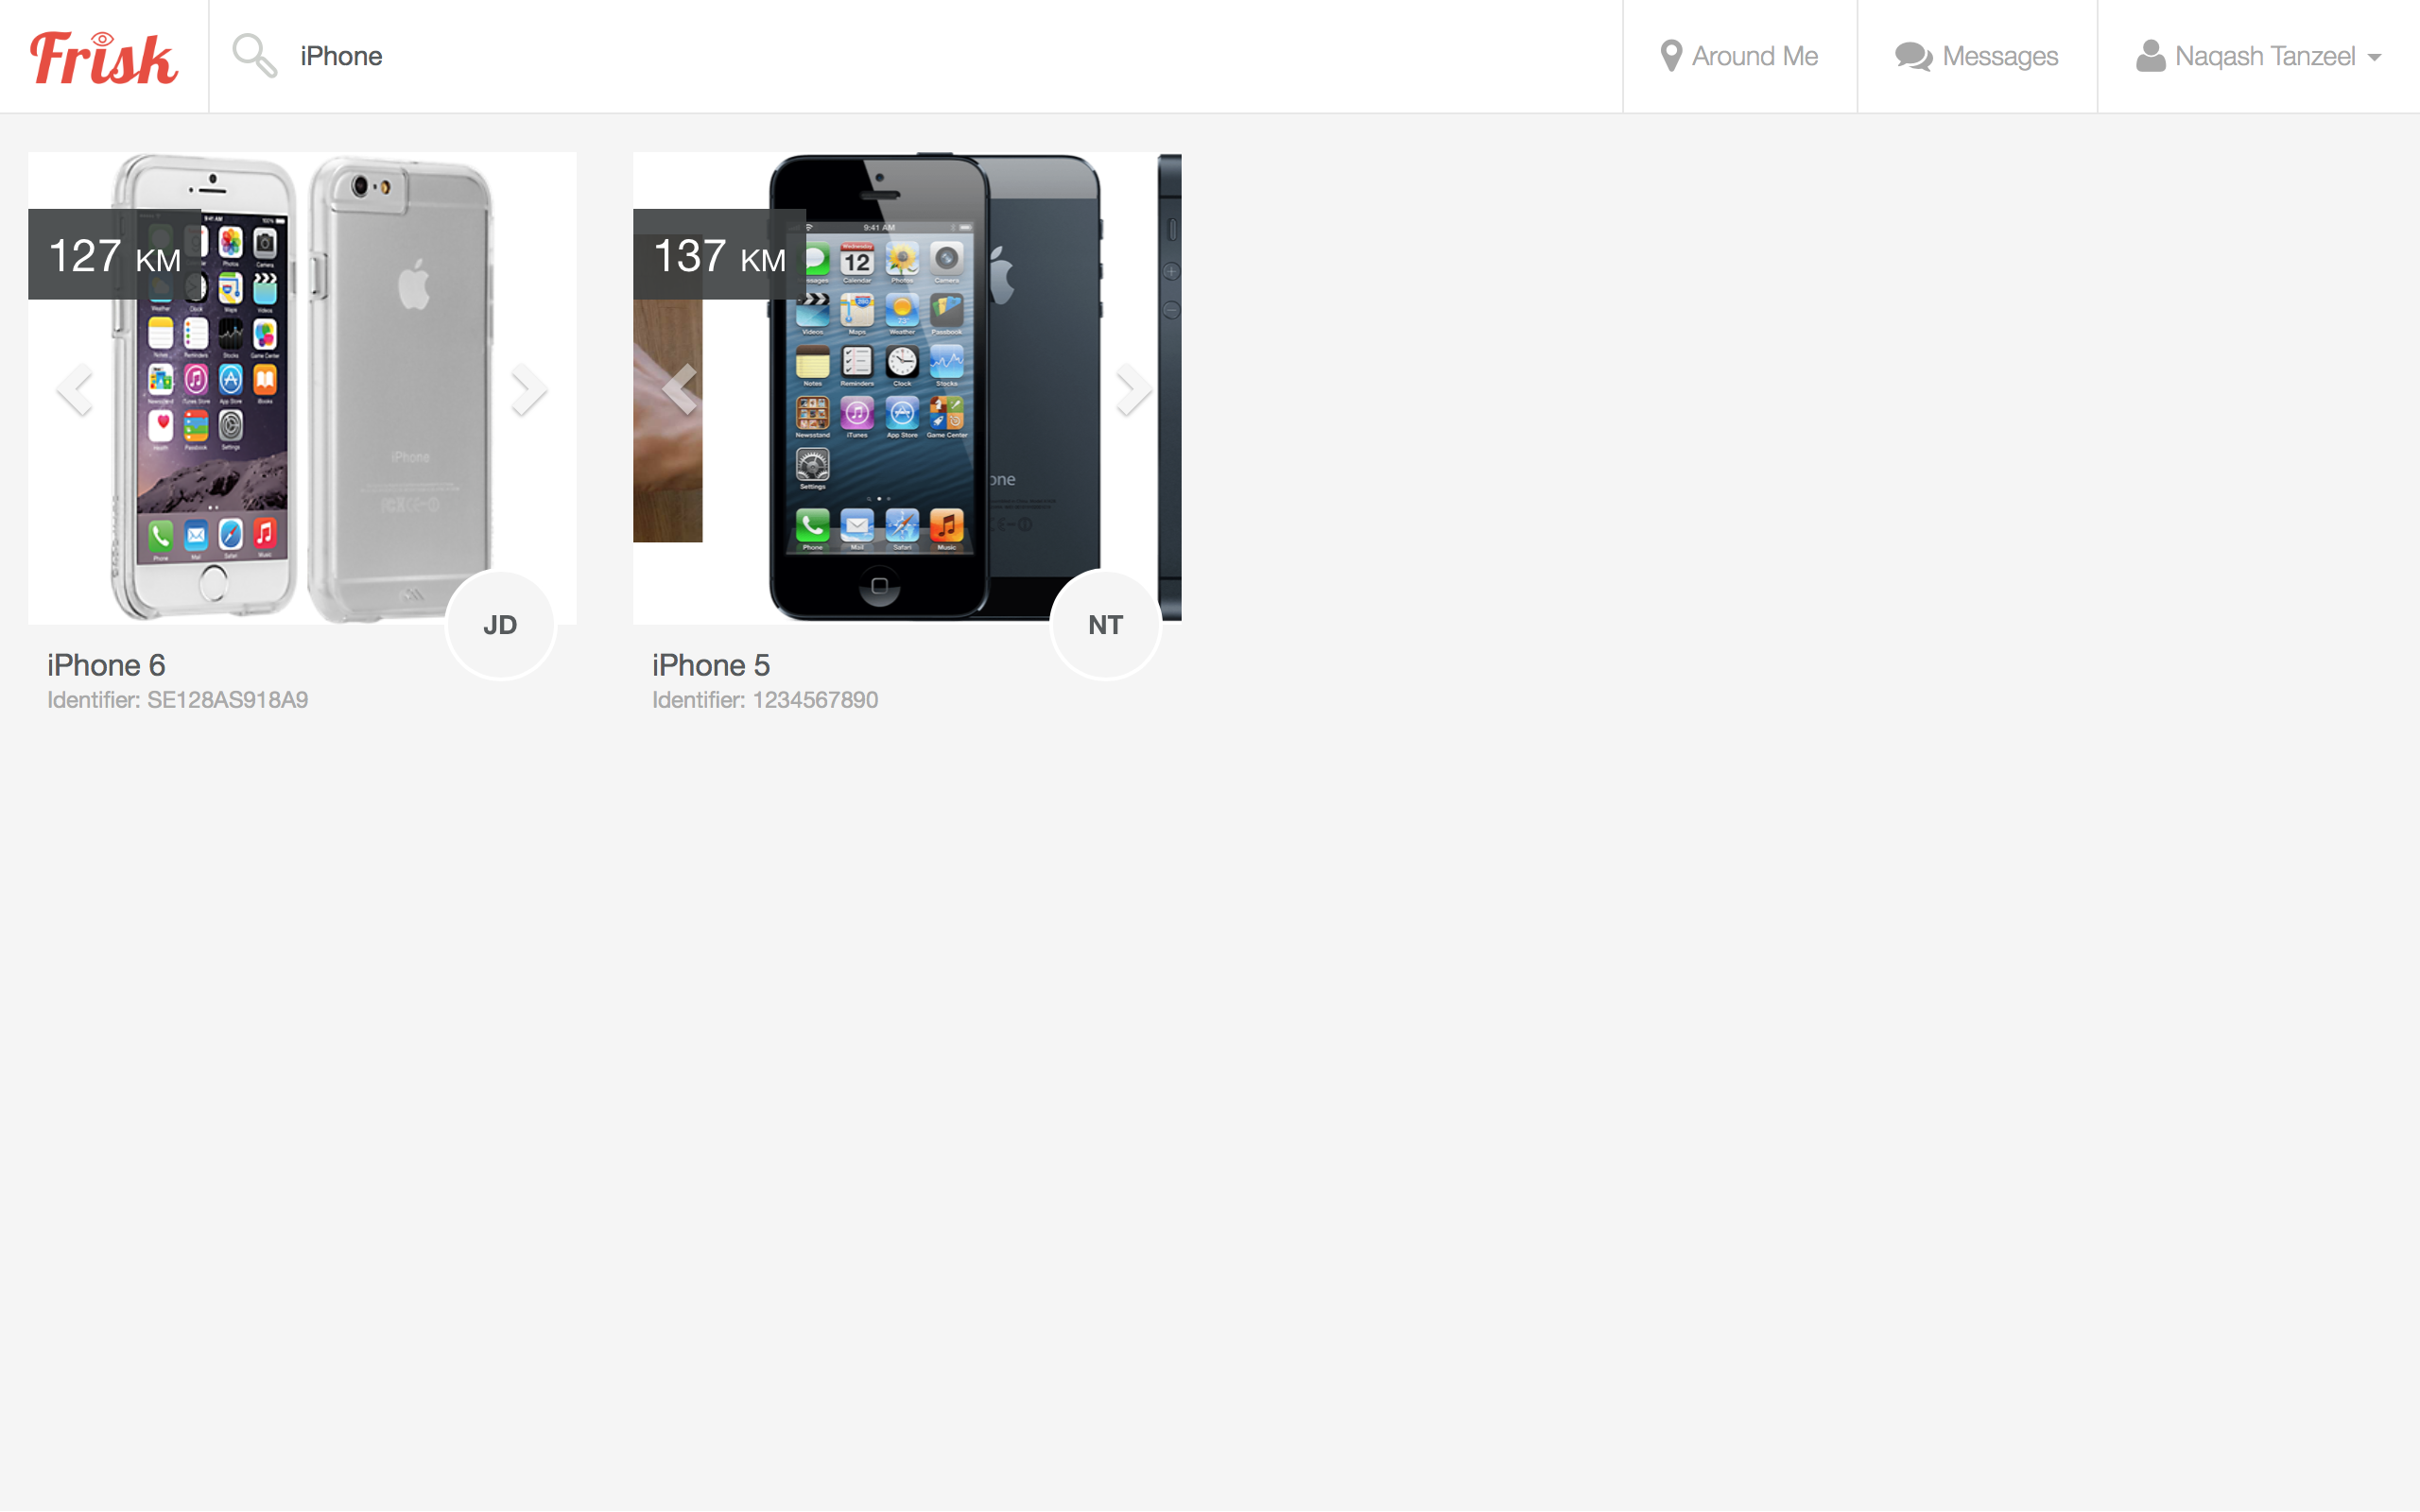
\includegraphics[width=1.0\textwidth]{images/Frisk/Page_Search}
	\caption{Frisk - Search Page} \label{fig:Page_Search}
\end{figure}

Figure \ref{fig:Page_Search} shows the search page with two results returned by the search query. The purpose of the search page is to display the search results for a query and additional details. As shows in the prototype, the result of the search are displayed as a grid. The original design for the search page displayed the results in a list view, which is the most common way of displaying results. After development commenced the design was updated and the grid approach was adopted as it allows the most of the information to be displayed without actually having to open the view item dialogue. The use of a grid view also allows for a slideshow of images to be displayed rather than a single cover image. Additionally the search page included a map in the original design, even though it was not a requirement, but this was removed as the search page can be viewed without providing the users location. This means that users can search for items without allowing access to their location and the functionality would not be limited, besides the removing of the distance label. The map may also lead to a more complex user experience as search may return results which may be located all over the country.

The search page will also allow the user to view more details about an item by clicking one of the results. This will either redirect the user to another page or present a popup containing full details about the item and how the user may contact the owner.

\subsubsection{Explore}

\begin{figure}[H]
	\centering
	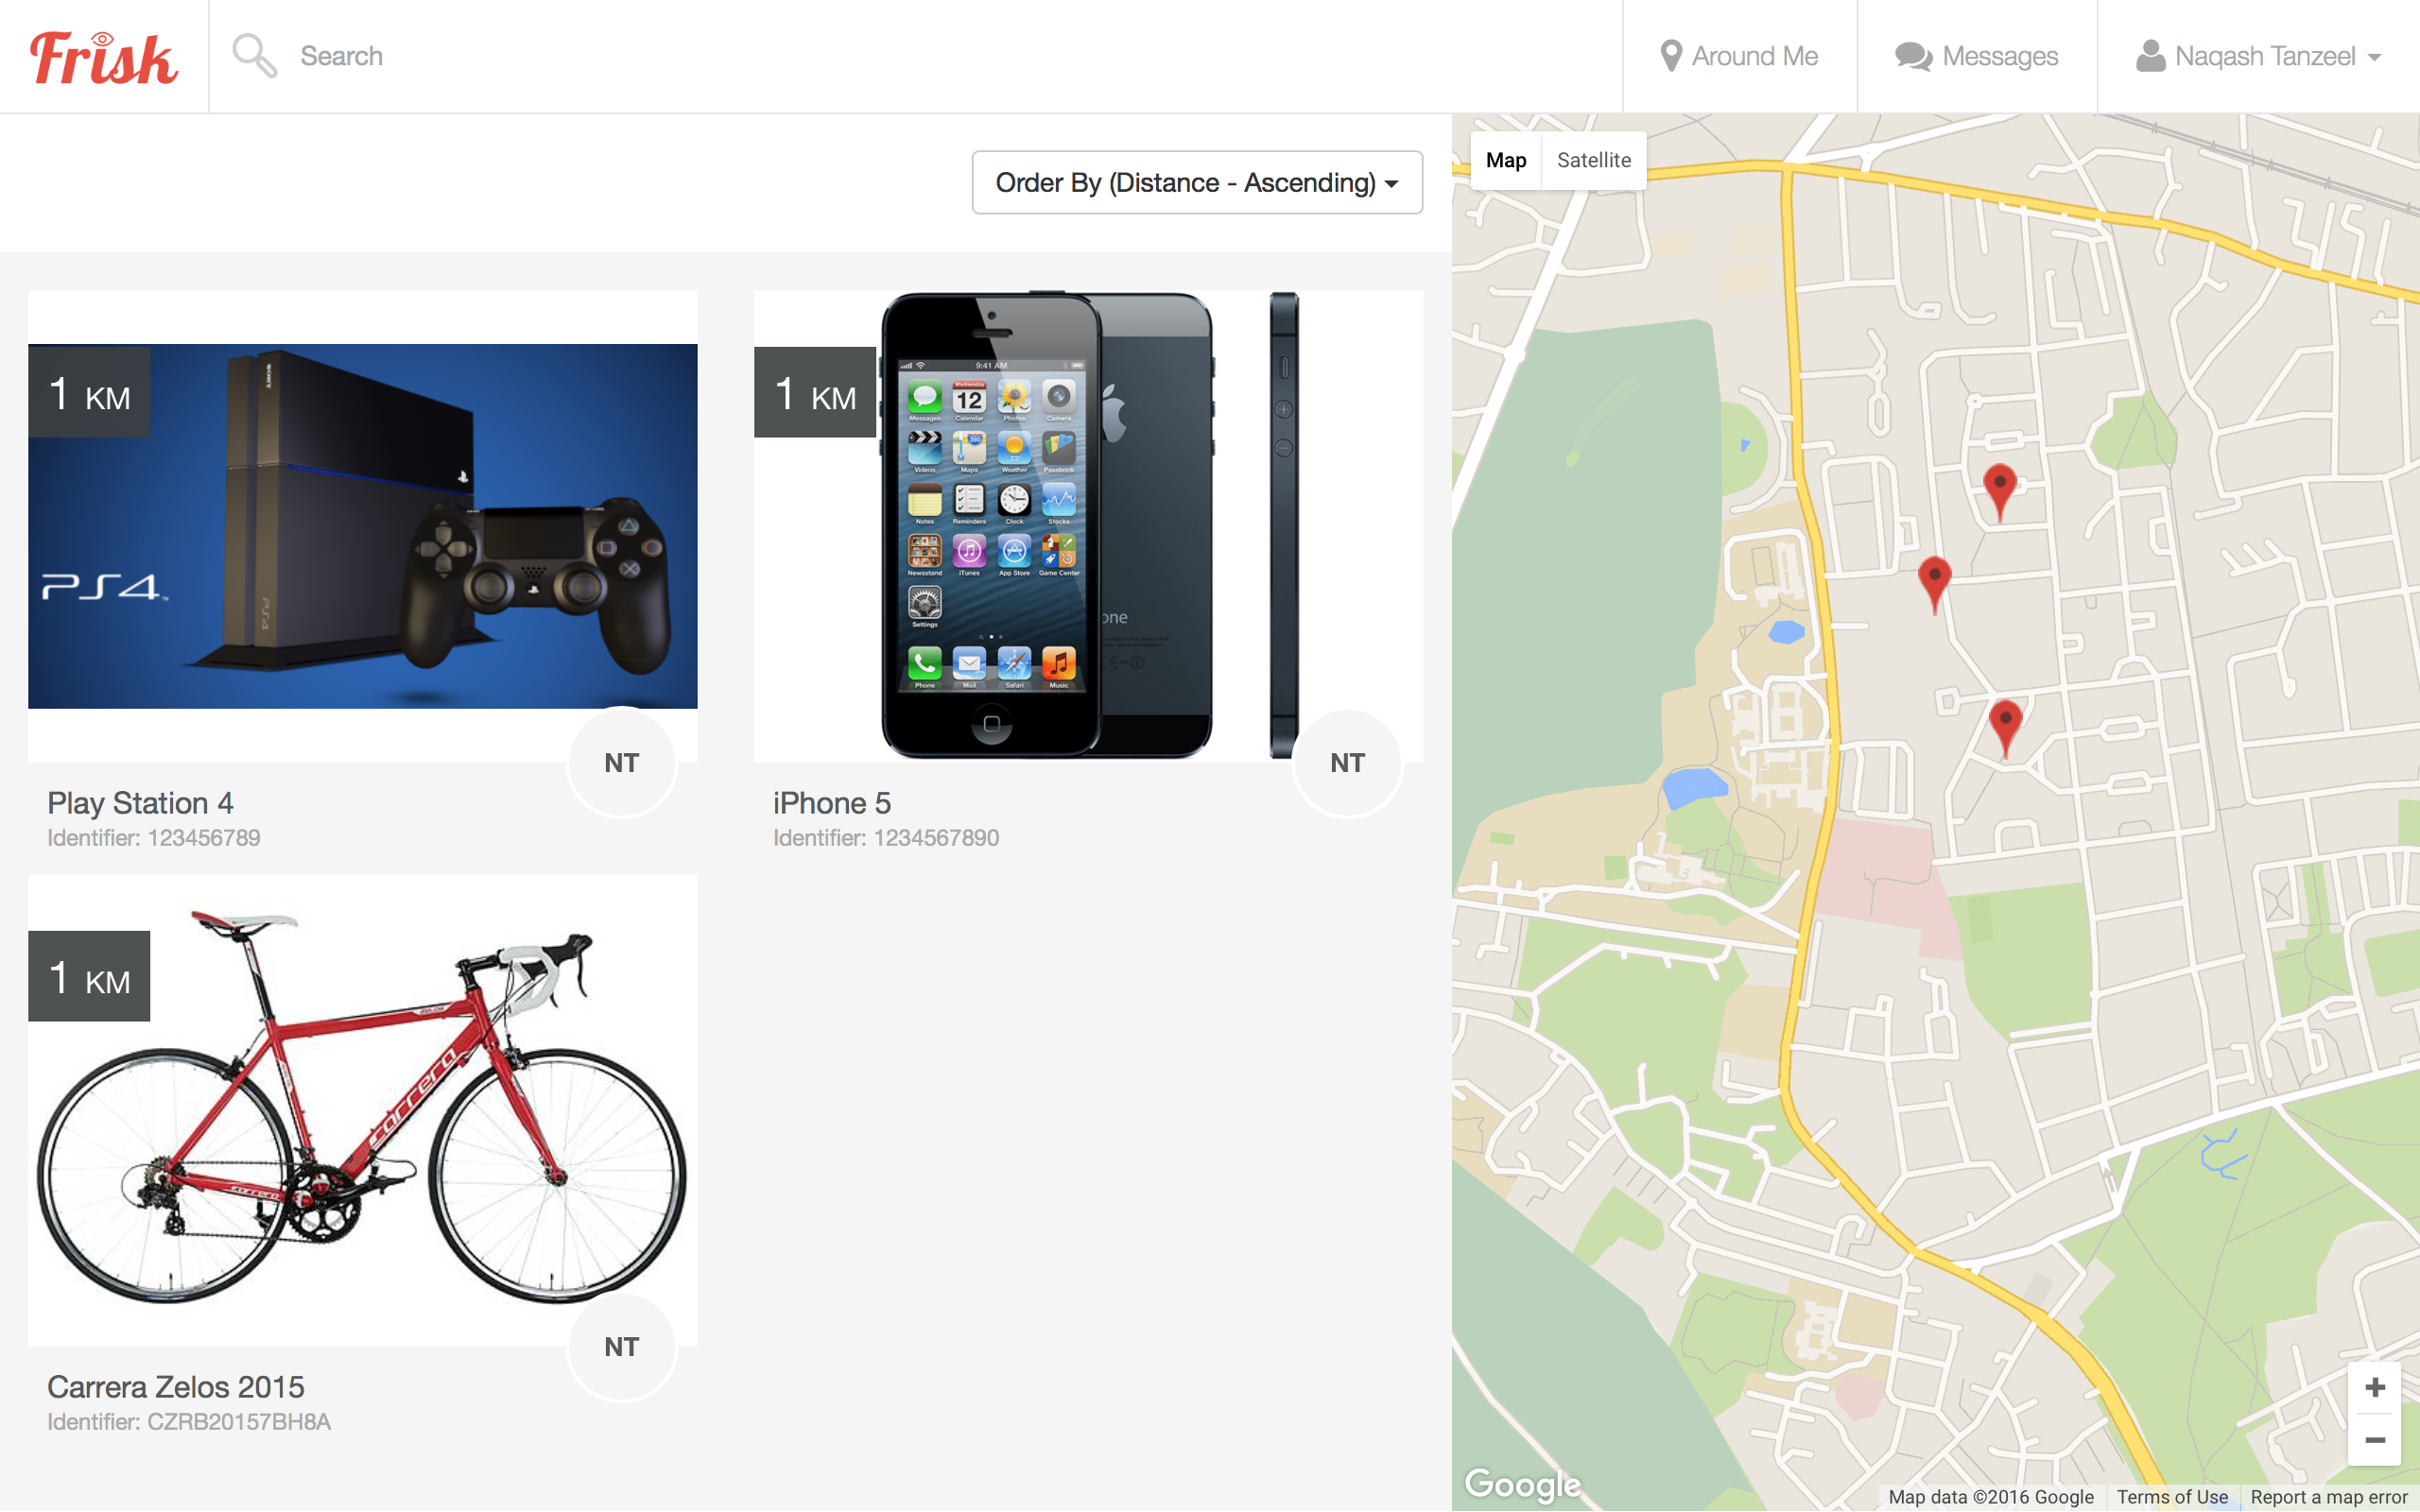
\includegraphics[width=1.0\textwidth]{images/Frisk/Page_Explore}
	\caption{Frisk - Explore Page} \label{fig:Page_Explore}
\end{figure}

The explore page provides one of the core features of the system. The purpose of the explore page is to allow users to see the items that have been reported as stolen in their local area. The page will display results in two separate views in contrast to the search page where results are only displayed in one view.

The first view, the grid view, will display the items in a similar way to the search page. Each result is a tile containing the details about an item. Once again, the user is able to view most the details, ranging from name to a slideshow of pictures, about the items in this view without having to click the item to load the view page. The purpose of this is to allow the user to quickly scroll through the result to find the item they're looking for. A sort feature will be provided on the explore page to aid this which will allow the user to sort the item by various attributes, such as name and distance. This can be achieved as the users location is required in order to access this page.

The second view, the map view, will display a map with markers for each item that has been reported as stolen. This view will allow the user to browse items by location, making it possible to see hotspots for theft and burglary. The map view will be visible alongside the gird view and the users can interact with it by dragging the map or clicking the markers. This functionality will however be limited to just desktop and larger screen devices such as tablets and will be hidden on mobile devices due to limited space.

\subsection{Dashboard Designs}
As discussed previously, a different approach was adopted for the design of the dashboard. The dashboard template consisted of a sidebar which contained the main navigation links. Additionally a navigation bar will be provided at the top of the page which will have a toggle to hide the sidebar, the page title, and optionally any actions that may be defined for the page. Each page can add actions to the navigation bar depending on the options available. This is followed by a crumb bar which build up links as the user navigates through sub pages. This allows the user to navigate back up the hierarchy to previous pages.

\subsubsection{Locations}

\begin{figure}[H]
	\centering
	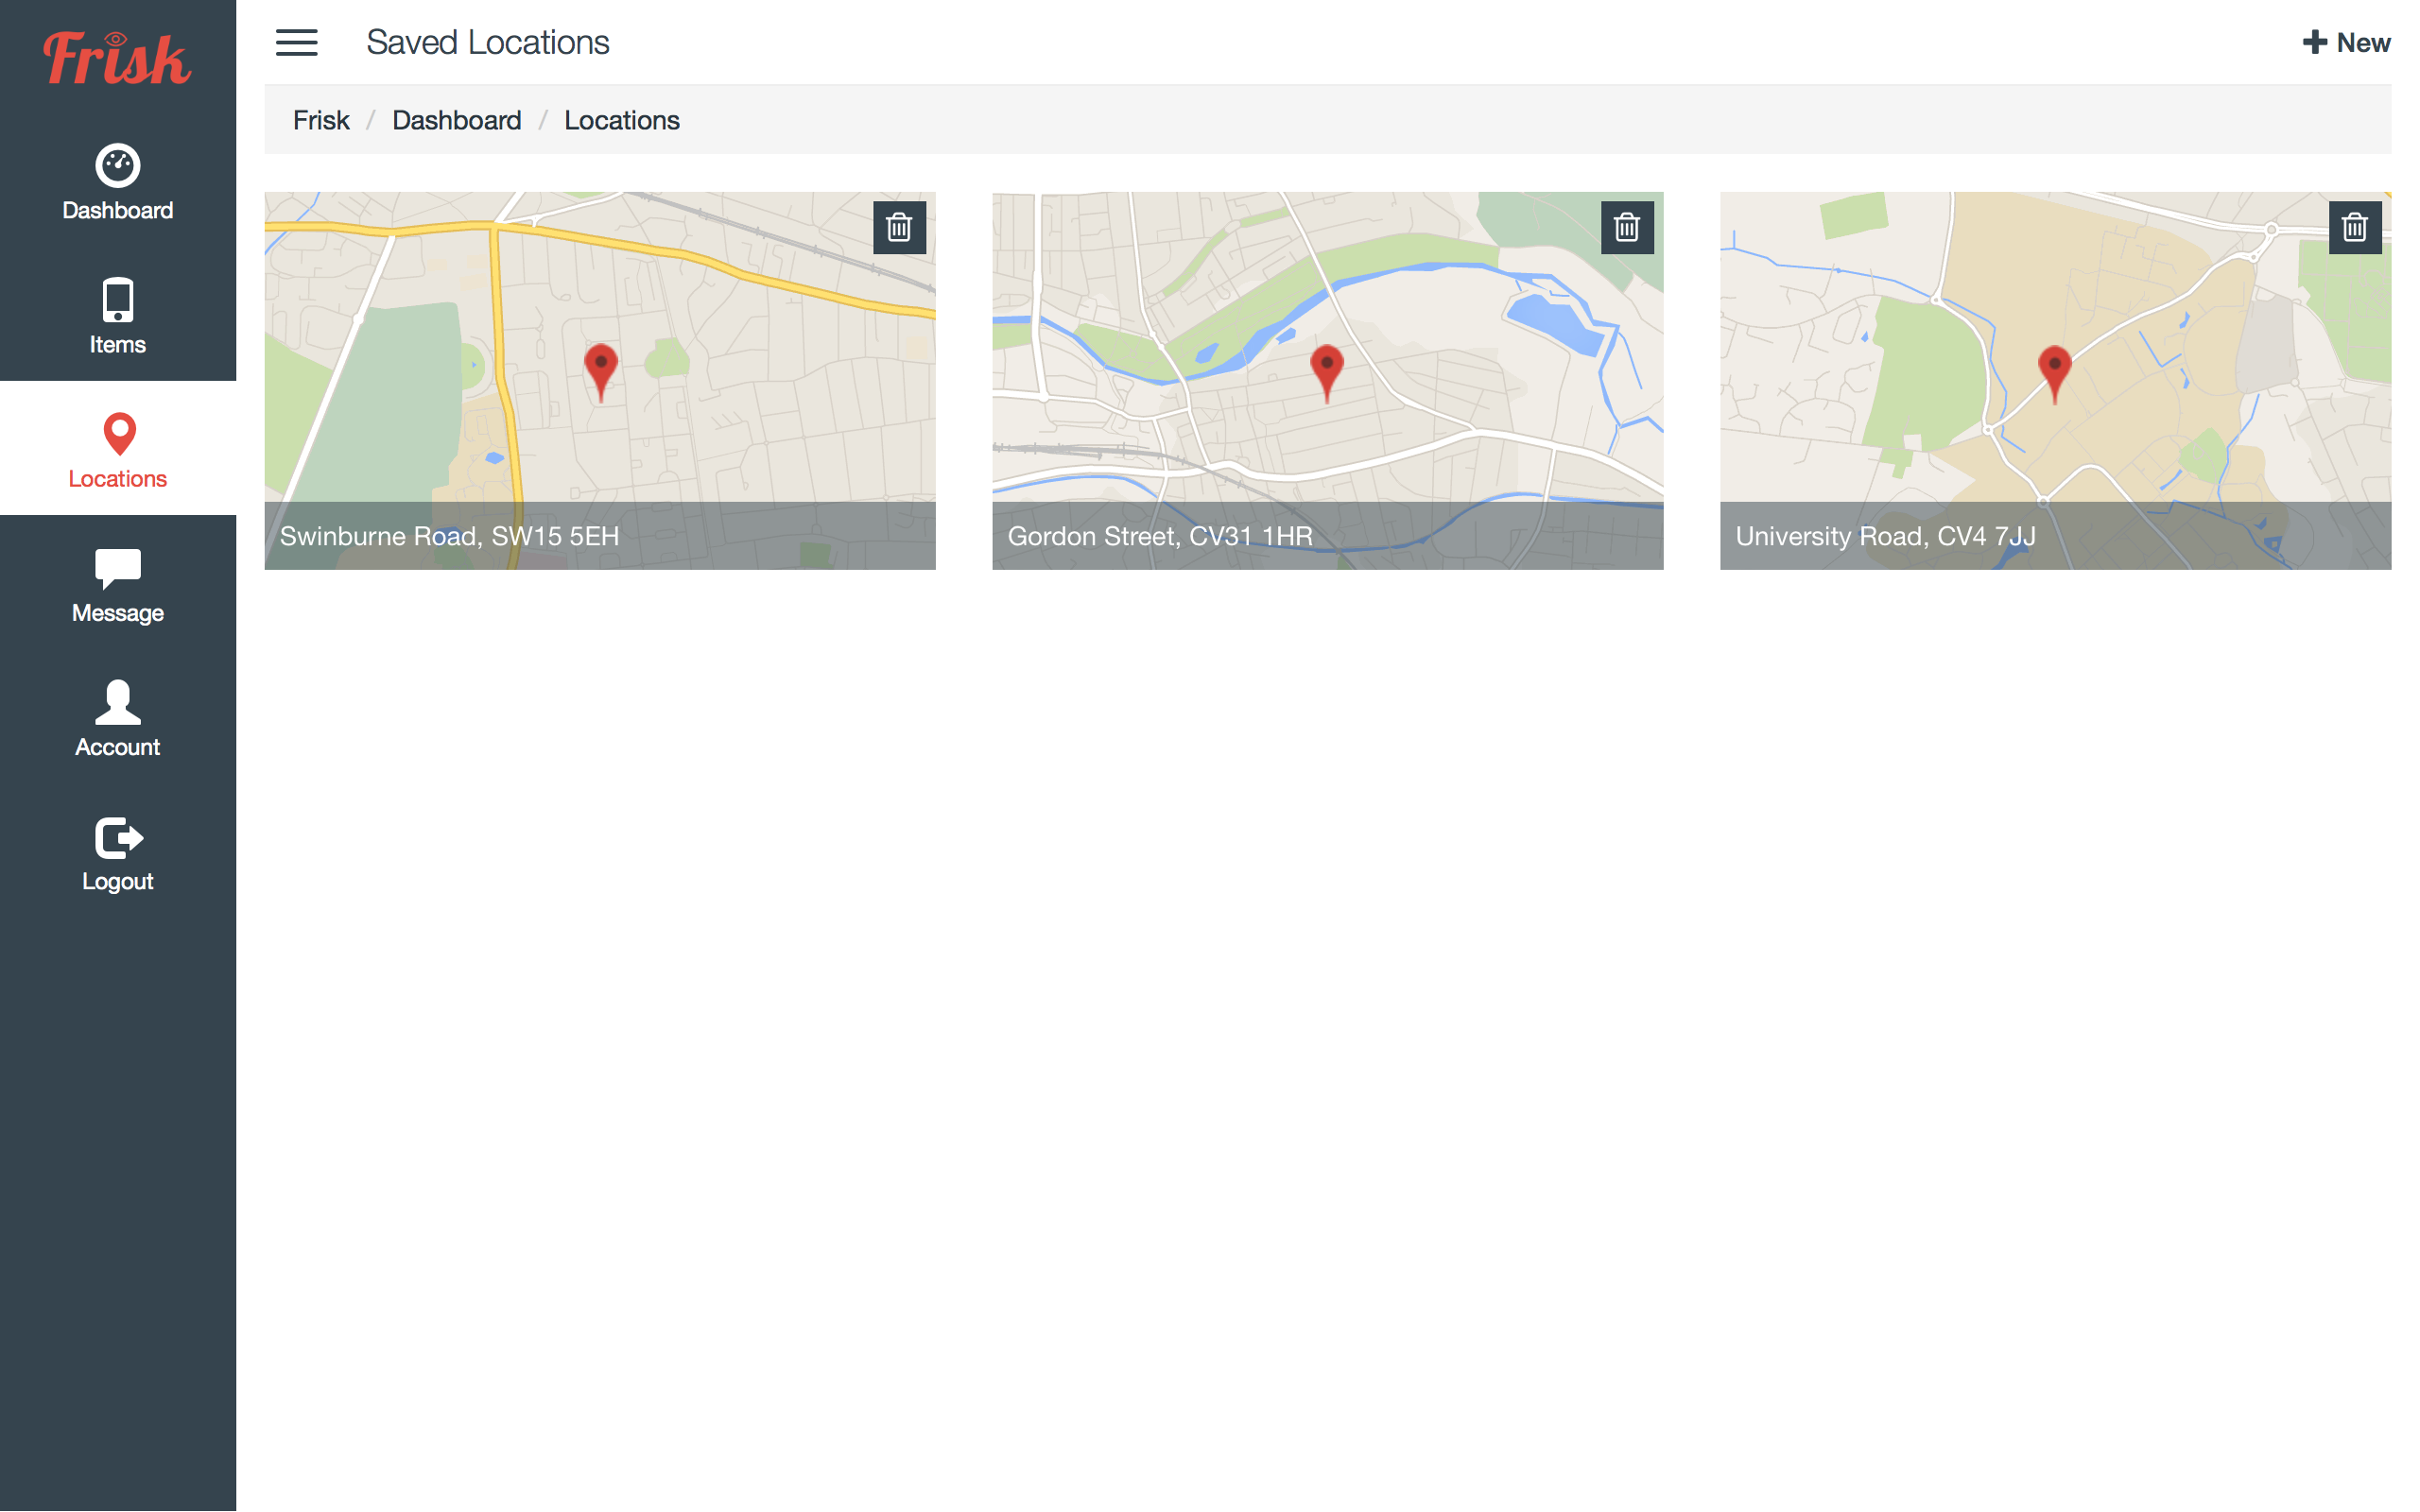
\includegraphics[width=1.0\textwidth]{images/Frisk/Dashboard_Locations}
	\caption{Frisk - Locations (Dashboard)} \label{fig:Dashboard_Locations}
\end{figure}

The locations page will be one of the first components to be built, as part of the dashboard, as this is one of the fundamental features in the system. The locations page will allow the user to view all the locations they have registered to their account. An initial design simply listed the locations in a table and the user would be able to delete these. In the later designs, it was decided the locations page will show a separate map with a marker for each location so the user can quickly identify each location. This can be seen in figure \ref{fig:Dashboard_Locations}. The locations page will also allow the user to register new location using a link provided in the navigation bar as well as remove any existing location using a delete button.

The creation of locations will also be accommodated by the locations page on the dashboard. A separate form was to be used to allow users to register location but a new design was proposed in which a popup will be presented. The user will be able to add new locations by completing the popup and they will be added in-line immediately. The implementation and design of this are discussed in section \ref{Section:Implementation}.

\subsubsection{Items}

\begin{figure}[H]
	\centering
	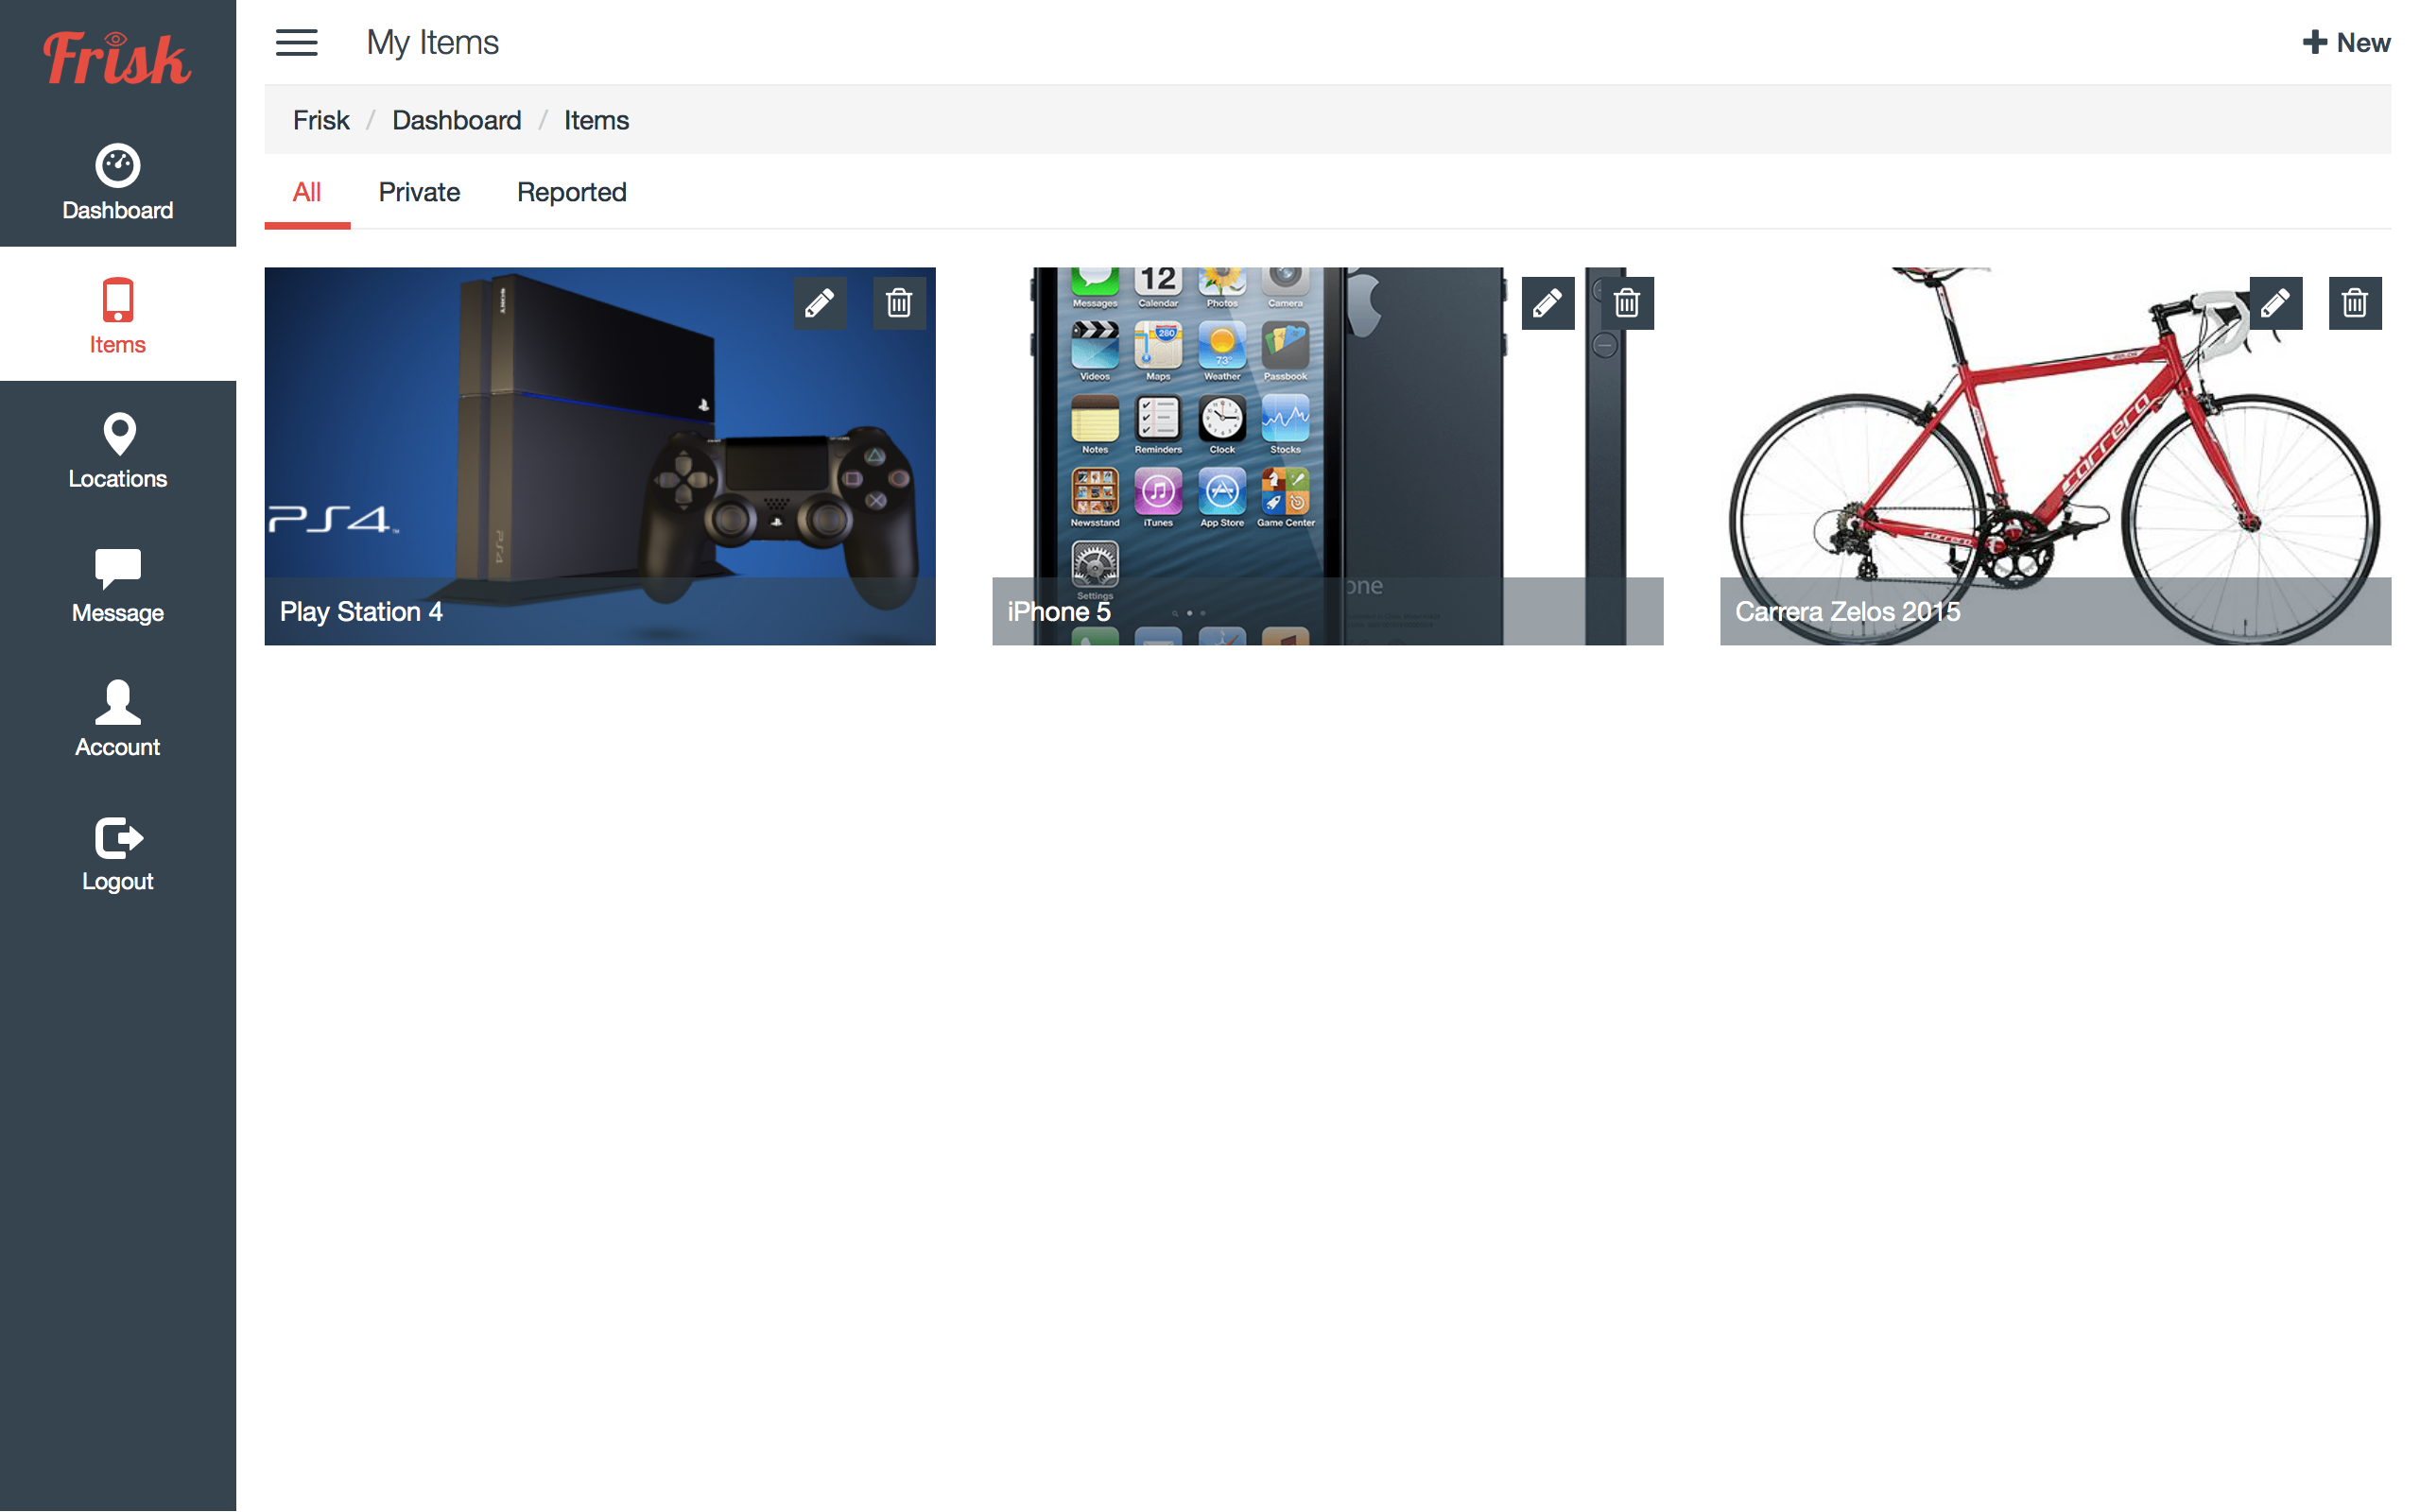
\includegraphics[width=1.0\textwidth]{images/Frisk/Dashboard_Items}
	\caption{Frisk - Items (Dashboard)} \label{fig:Dashboard_Items}
\end{figure}

The items page in the dashboard allows the user to manage all the items registered to their account. The items are split up into three categories. The user will be able to switch between these categories using simple tabs or links and the results will be updated without refreshing the page. Each item will be displayed as a tile with minimal detail, an image and the name of the item. Each tile will contain a set of actions, similar to locations, these will allow the user to edit or delete that specific item, shown in figure \ref{fig:Dashboard_Items}.

A ``new'' link will be provided in the navigation to allow the user to register new items. Creating of items is implemented as a simple form, shown in figure \ref{fig:Dashboard_Create_Item}. The same form is utilised for editing items but the cover image field is hidden.

\begin{figure}[H]
	\centering
	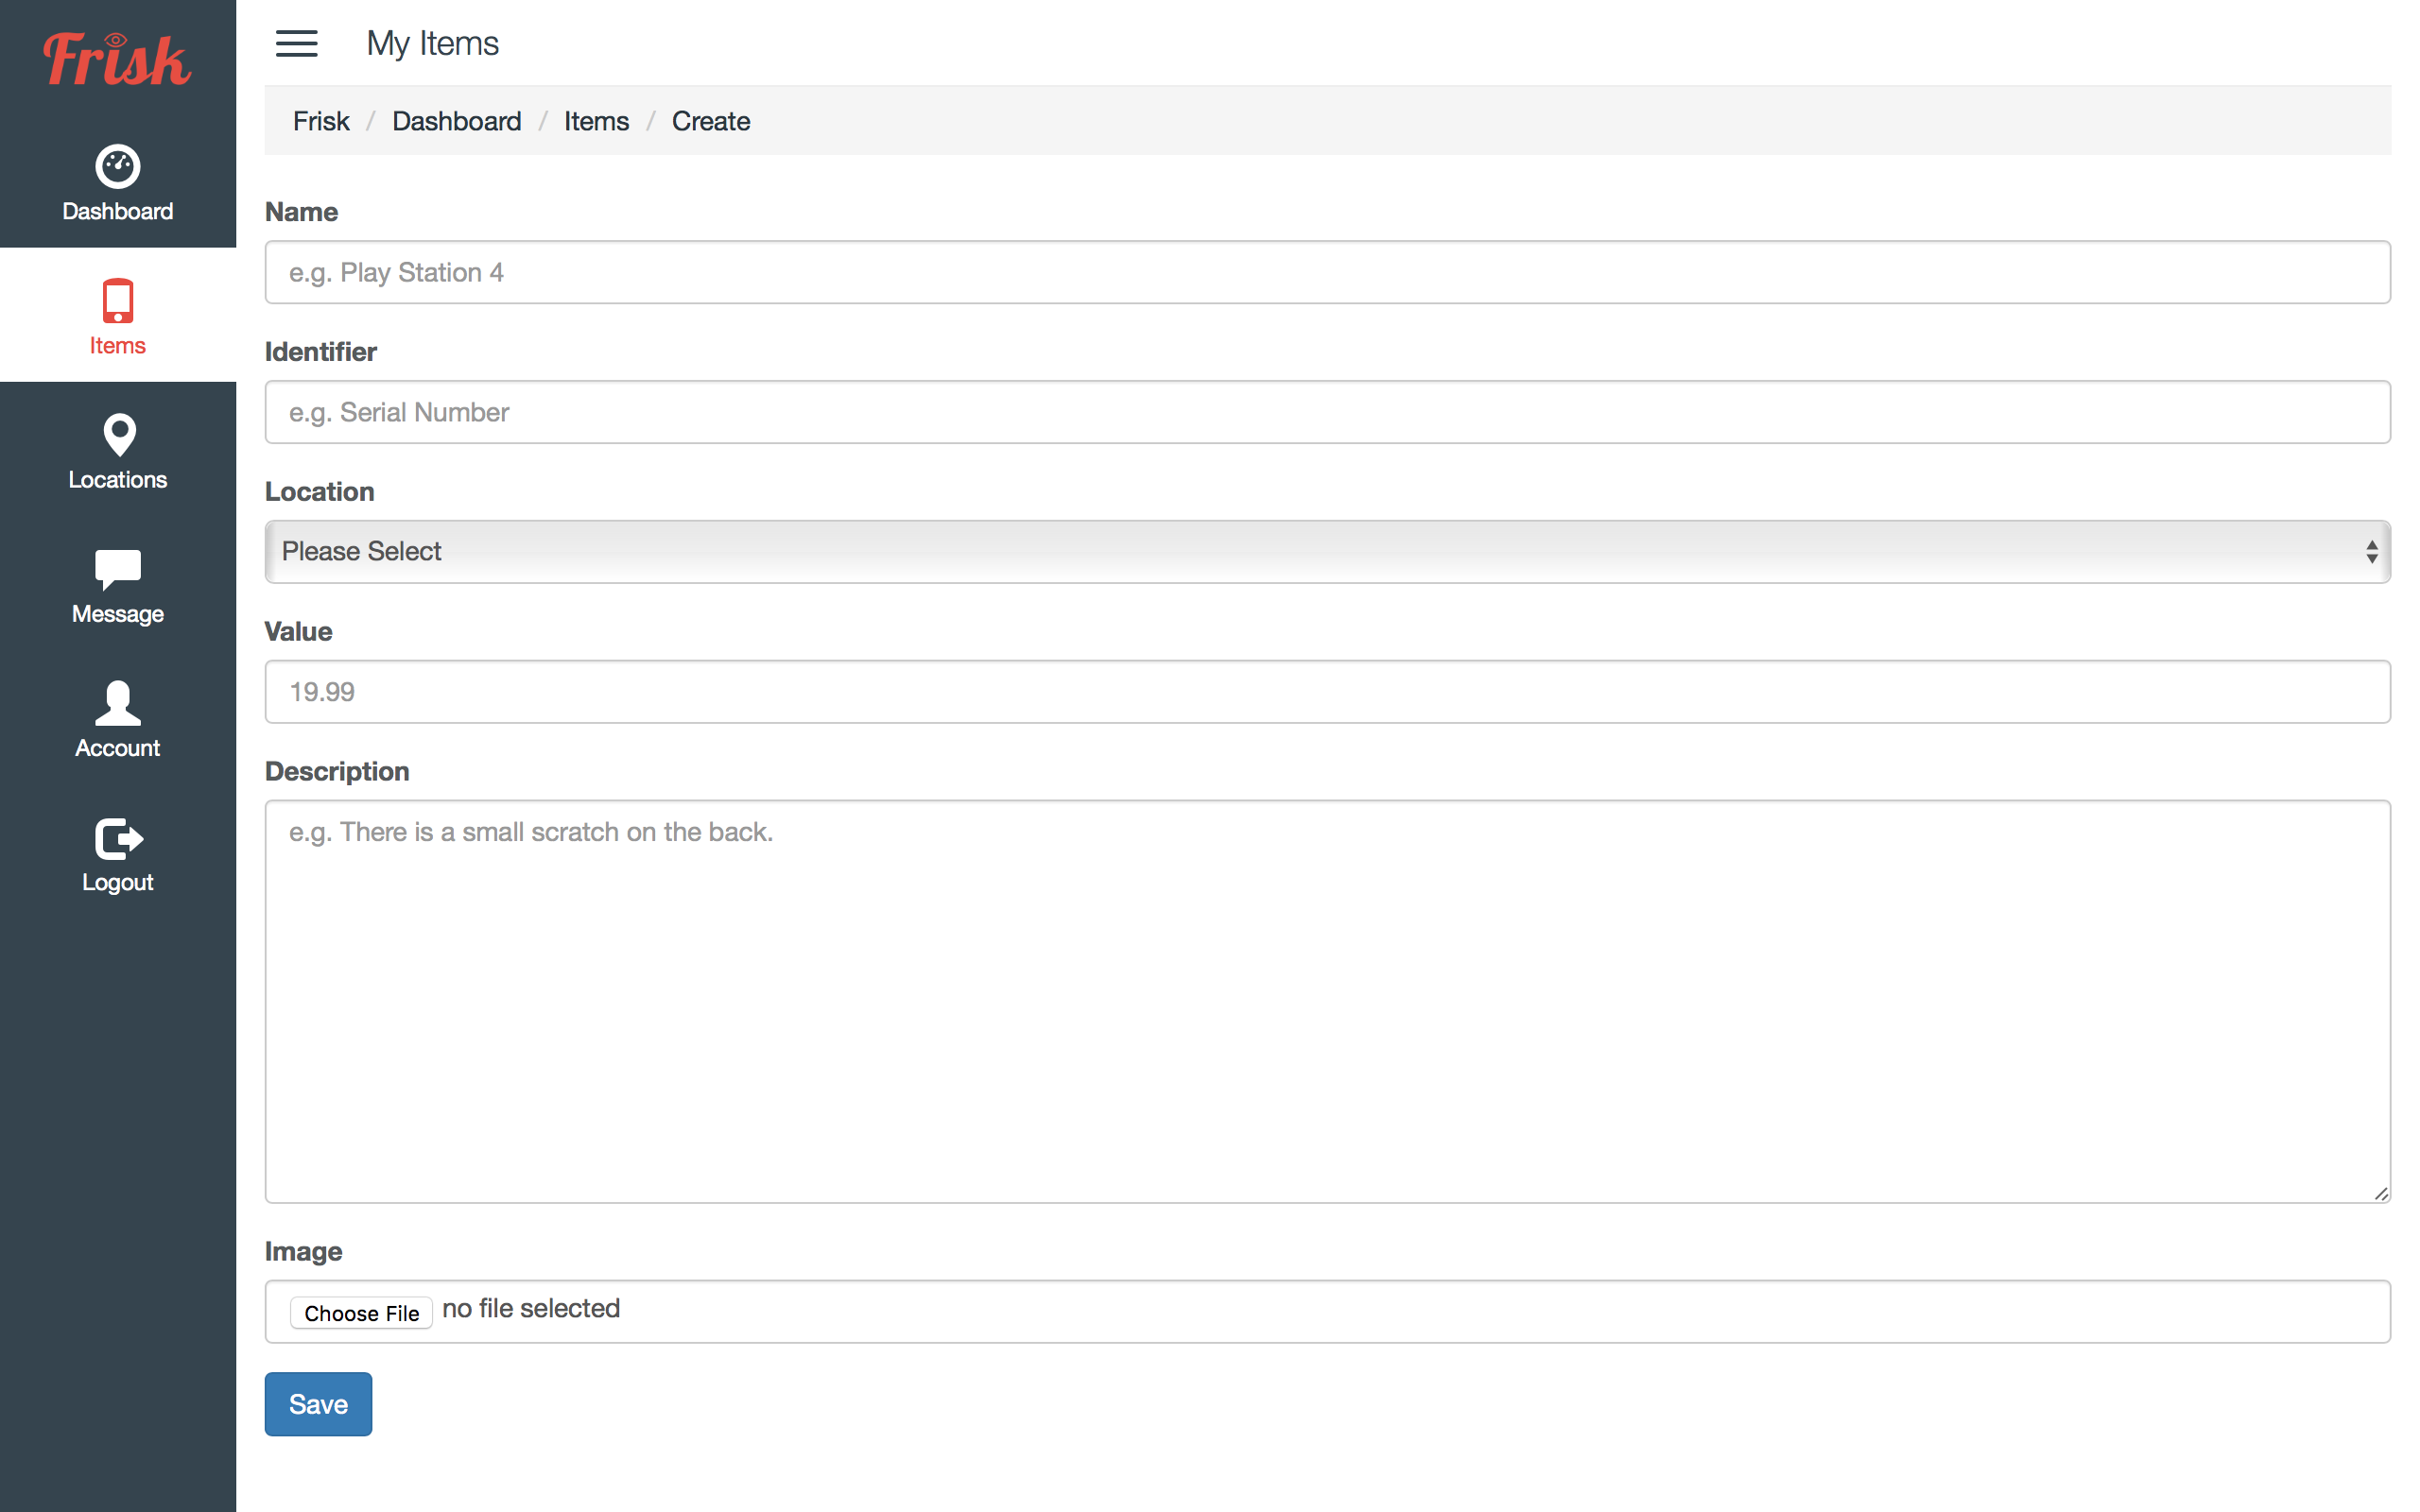
\includegraphics[width=1.0\textwidth]{images/Frisk/Dashboard_Create_Item}
	\caption{Frisk - Create or Edit Item (Dashboard)} \label{fig:Dashboard_Create_Item}
\end{figure}

\begin{figure}[H]
	\centering
	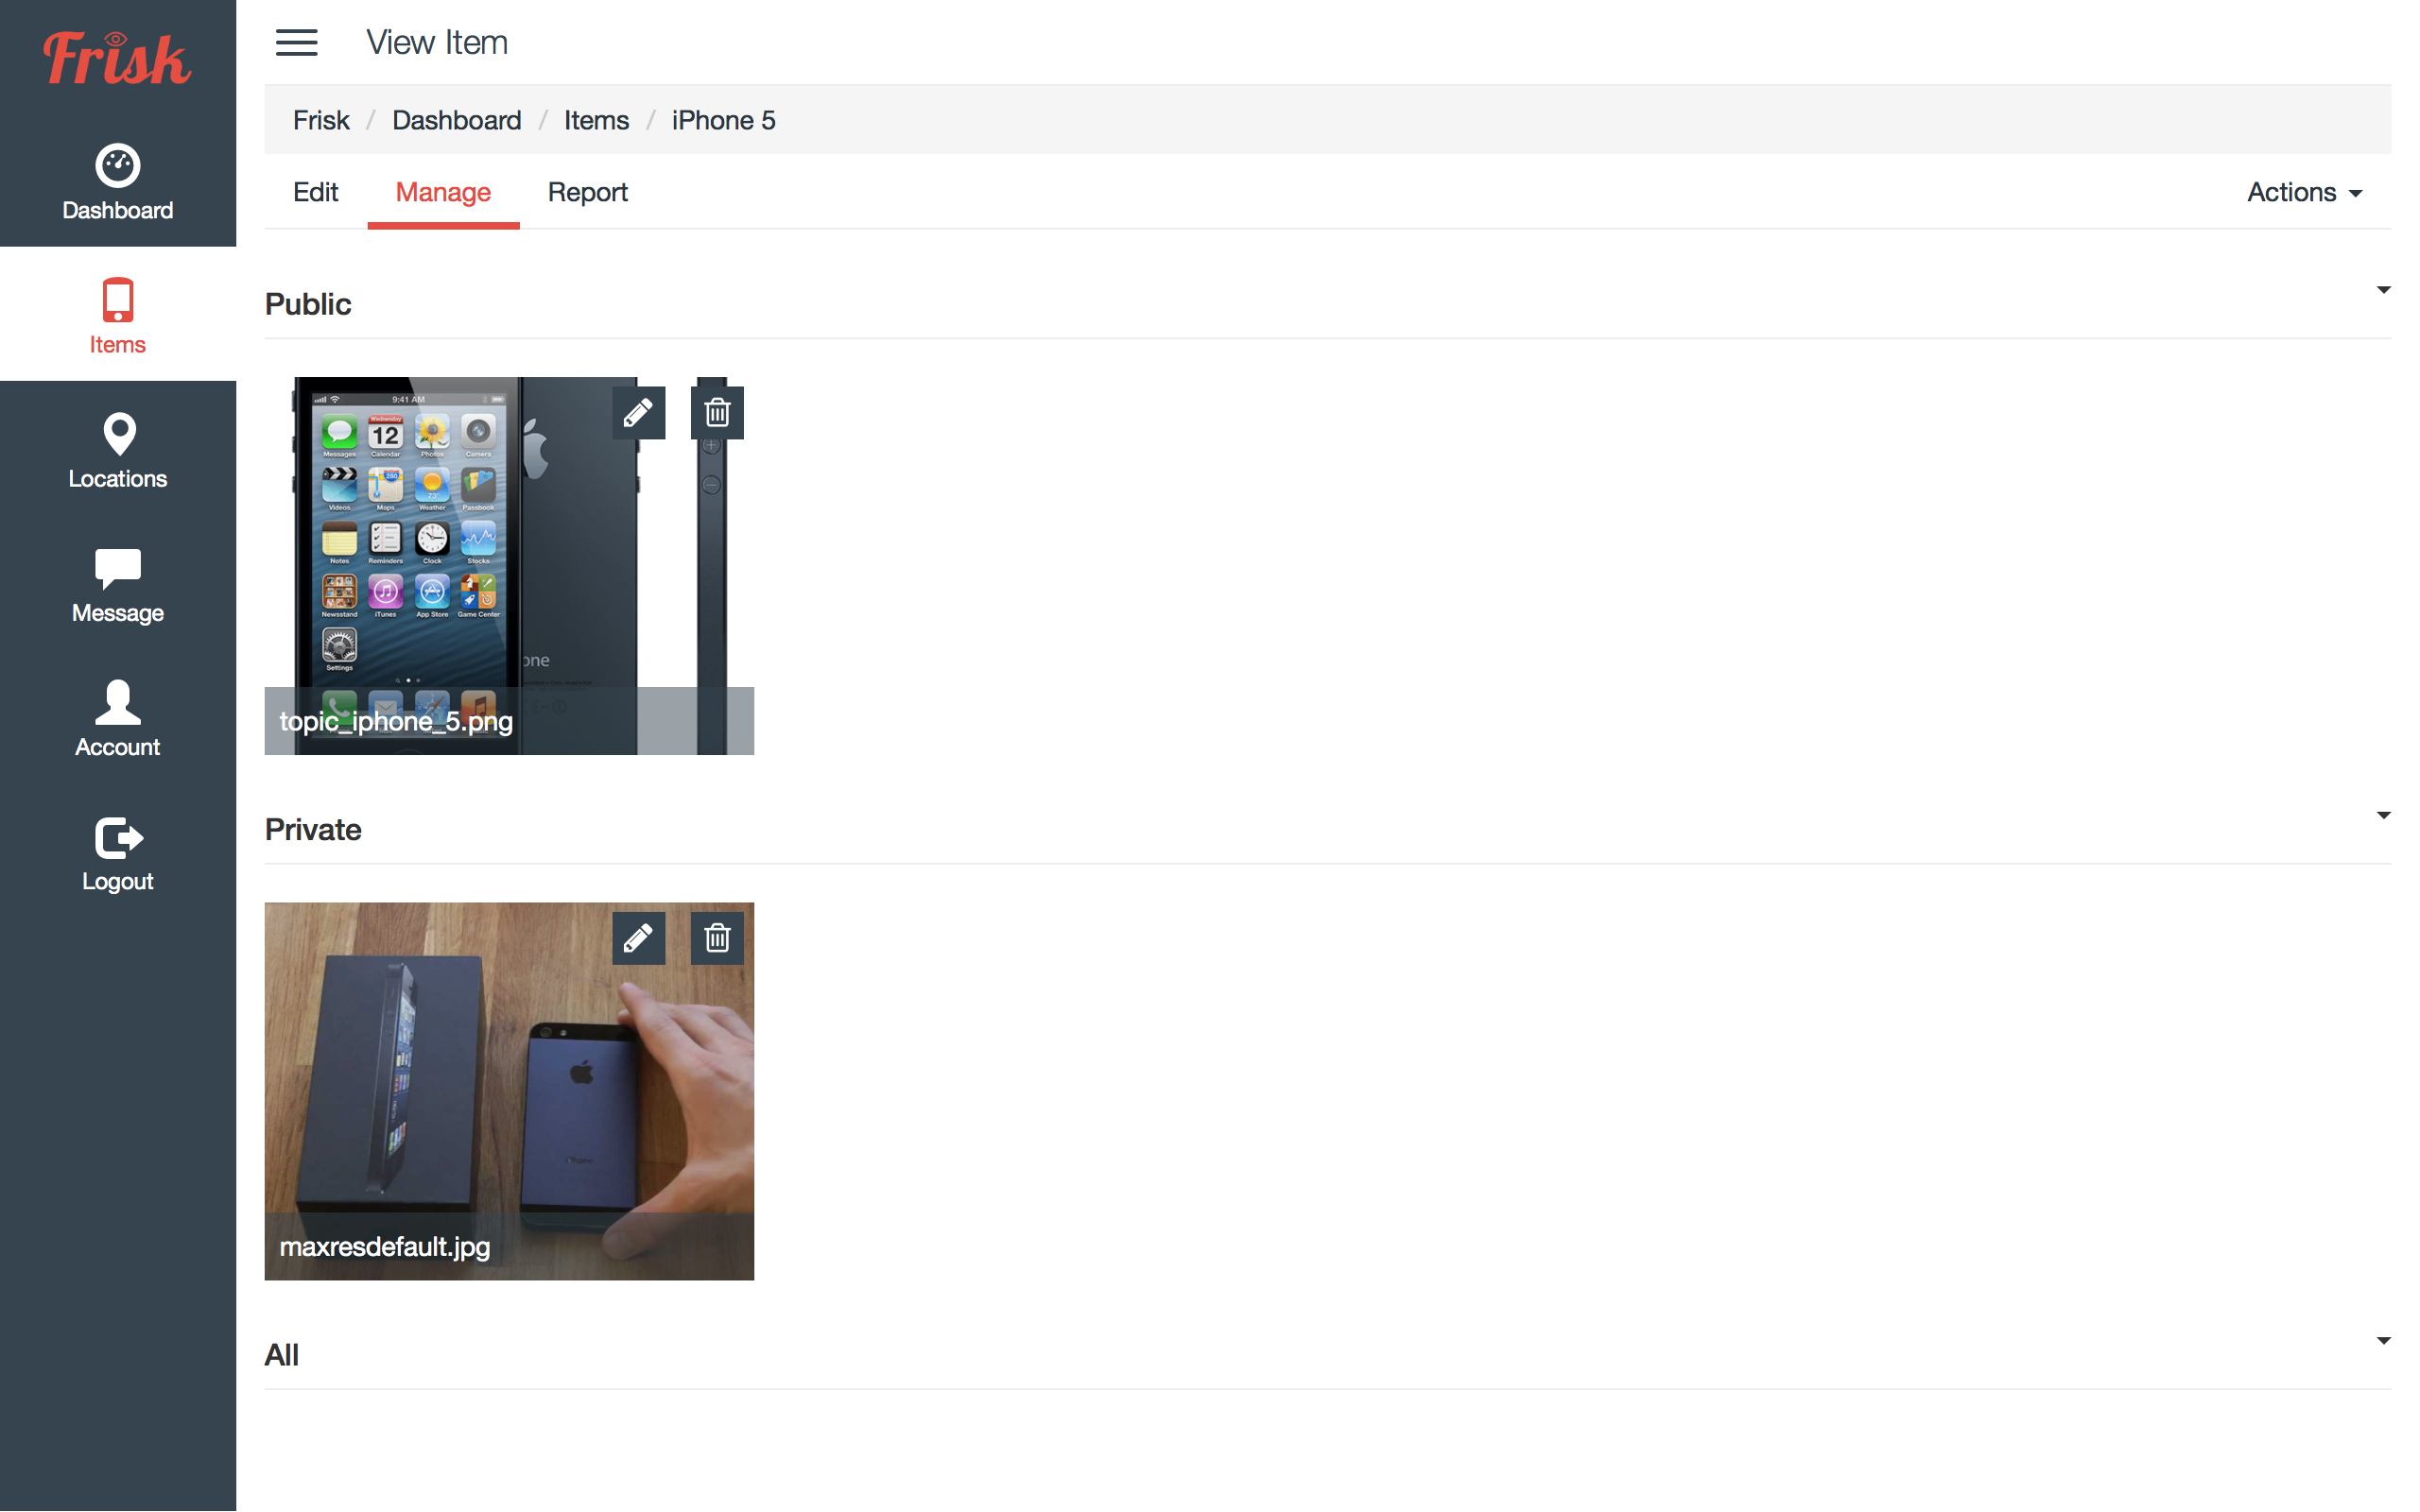
\includegraphics[width=1.0\textwidth]{images/Frisk/Dashboard_Resources}
	\caption{Frisk - Item Resources (Dashboard)} \label{fig:Dashboard_Resources}
\end{figure}

The resources page is essentially a part of the items component as resources are associated with an item in contract with locations which are independent but may be associated with an item. The main purpose of the resources page is to allow the user to manage the resources for an item which includes creating, editing, toggling publicity, and deleting. In order to access the resources page, the user will first navigate to the edit item page where the resources page where will be provided as a tab below the crumb bar. This can be seen in figure \ref{fig:Dashboard_Resources}.

On the resources page, the resources will again be visible as tiles containing an image and the alias set by the user. Once again, the resources are split into three categories as shown in figure \ref{fig:Dashboard_Resources}. The user can choose to expand or hide any one of the categories by simply clicking the heading. The user will be able to edit or delete a resource using the links provided. The creation and editing of resources will provided either inline or as a popup and is discussed further in section \ref{Section:Implementation} where the implementation details are provided.

\subsubsection{Messages}

\begin{figure}[H]
	\centering
	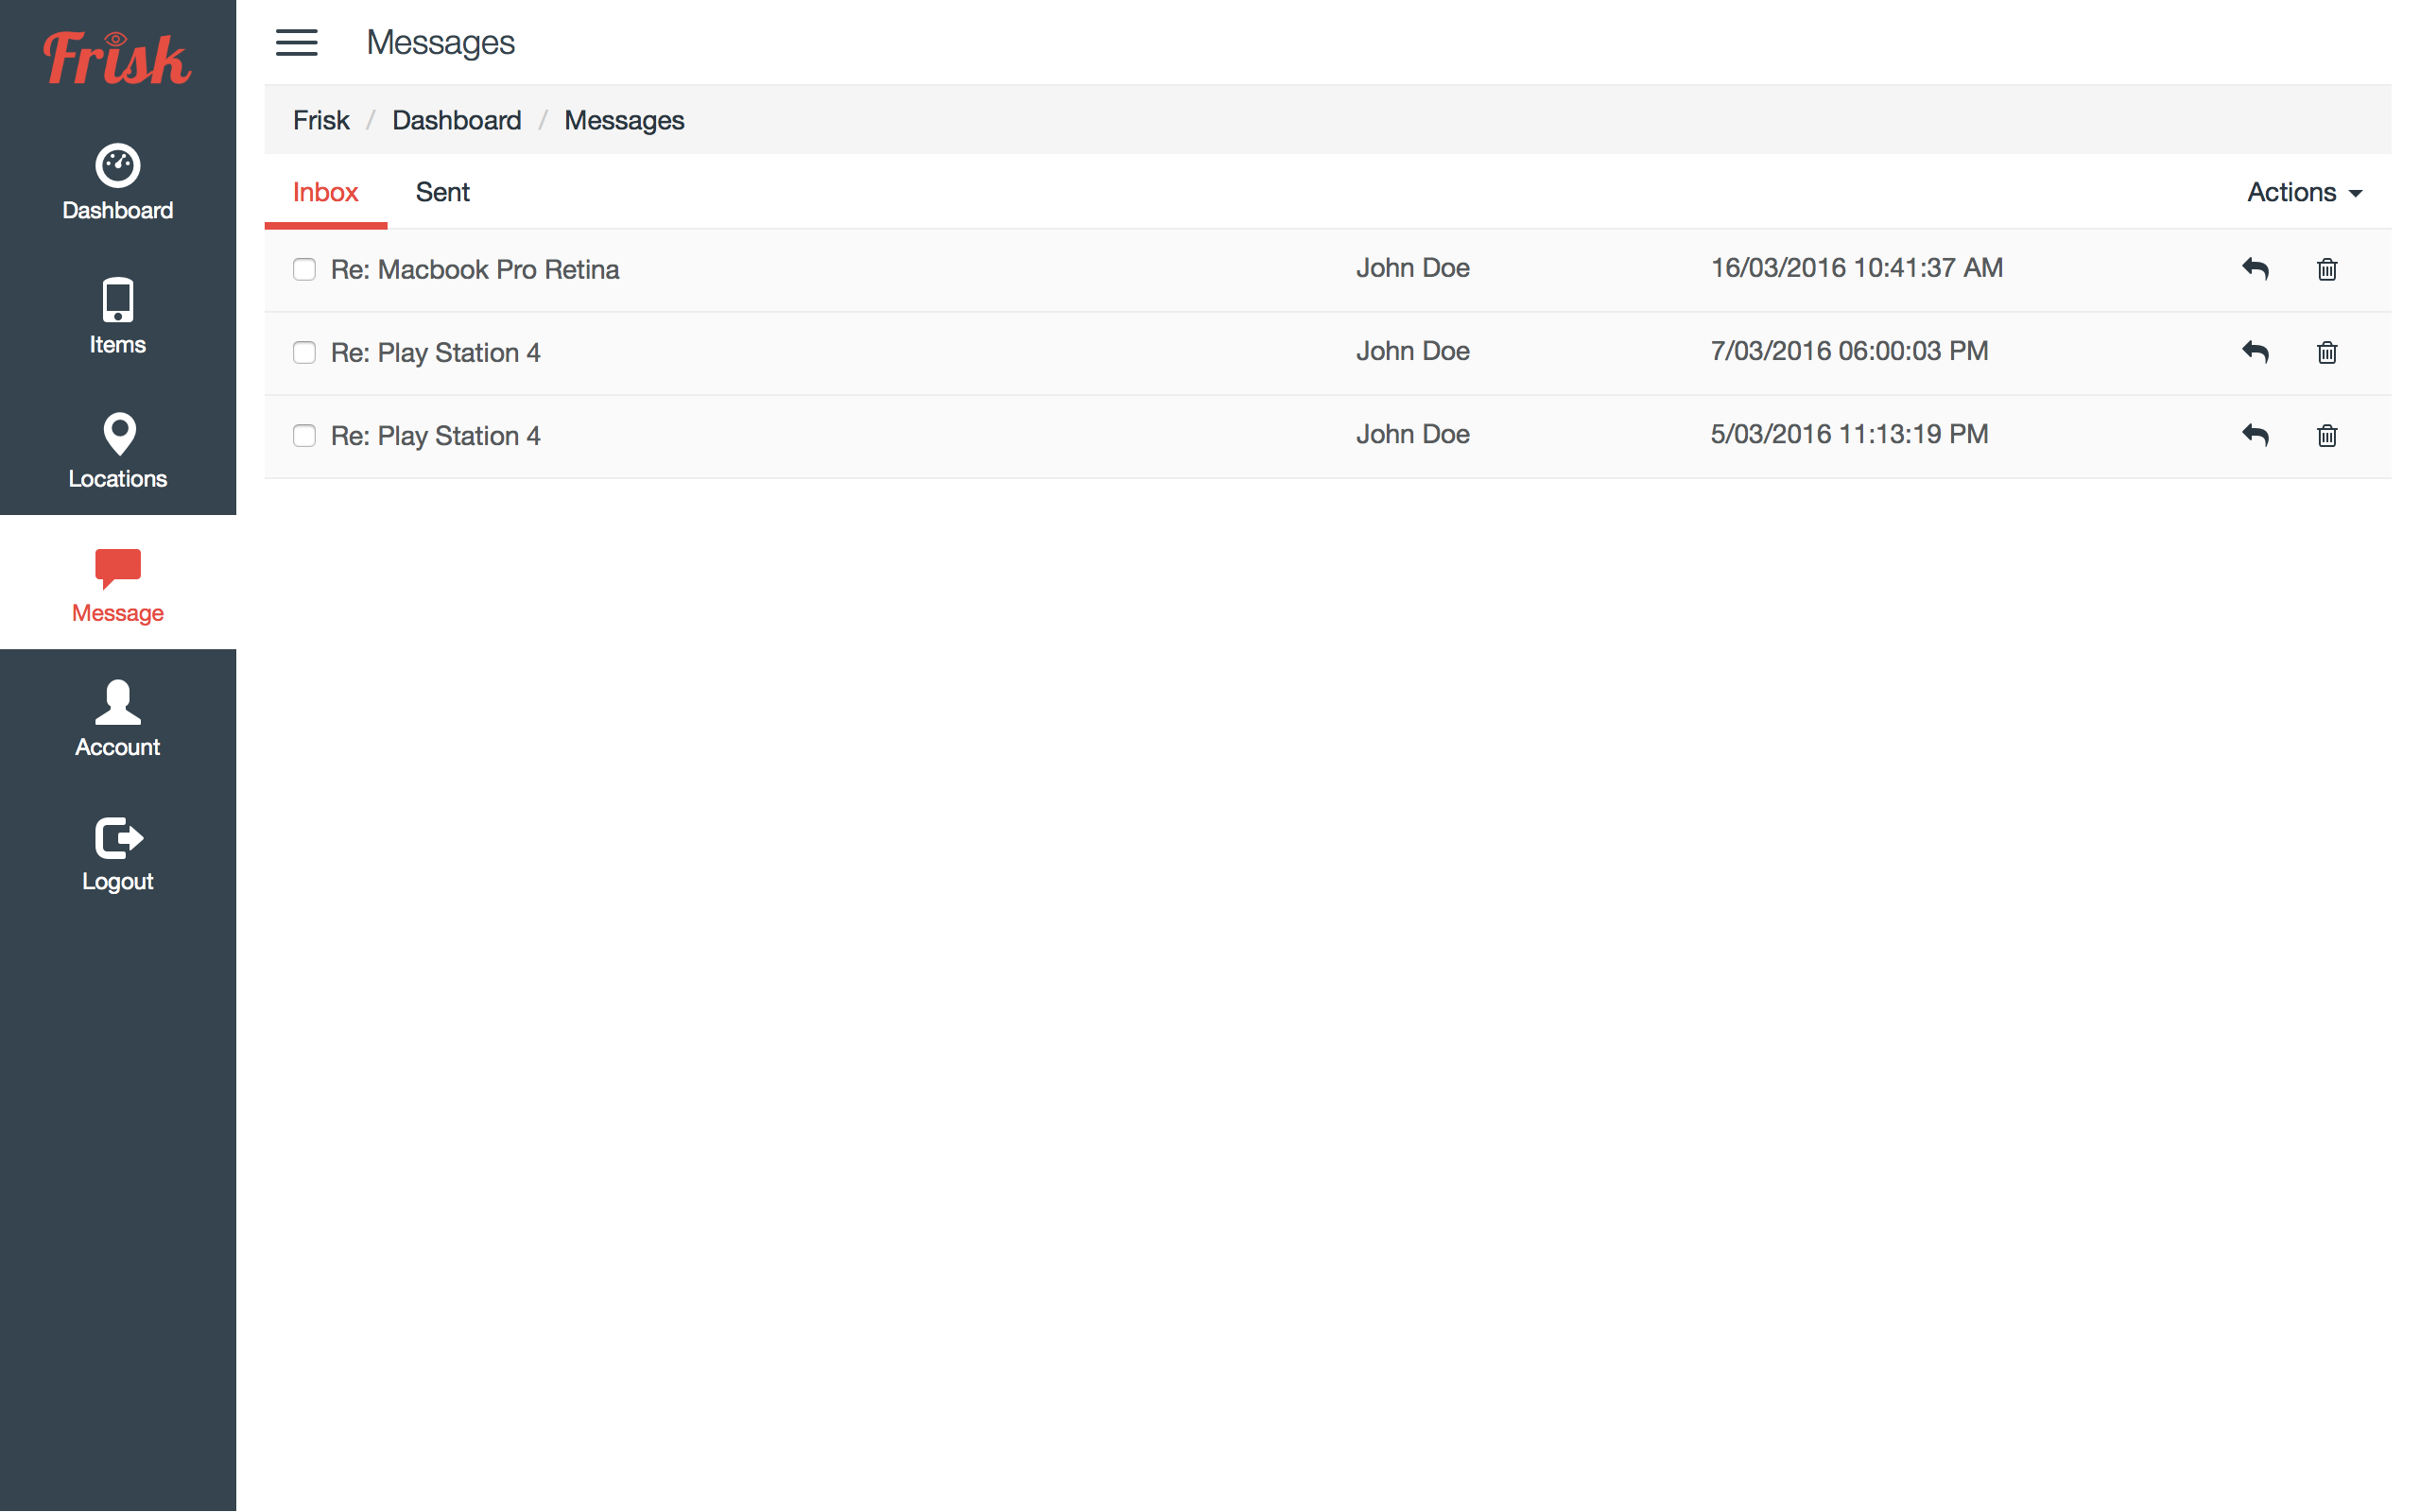
\includegraphics[width=1.0\textwidth]{images/Frisk/Dashboard_Messages}
	\caption{Frisk - Messages (Dashboard) } \label{fig:Dashboard_Messages}
\end{figure}

The messages section of the dashboard will provide an email system like experience to the user. The page will provide the standard dashboard template but in addition to this the user will be able to able to switch between their received and sent messages using a tab like interface just below the crumb bar (See figure \ref{fig:Dashboard_Messages}). The messages will be displayed in a list or table format as shown in figure \ref{fig:Dashboard_Messages}. The unread messages will be highlighted in bold whereas the read messages will be displayed in standard format. Links will be provided to allow the user to reply to to or delete messages.


\begin{figure}[H]
	\centering
	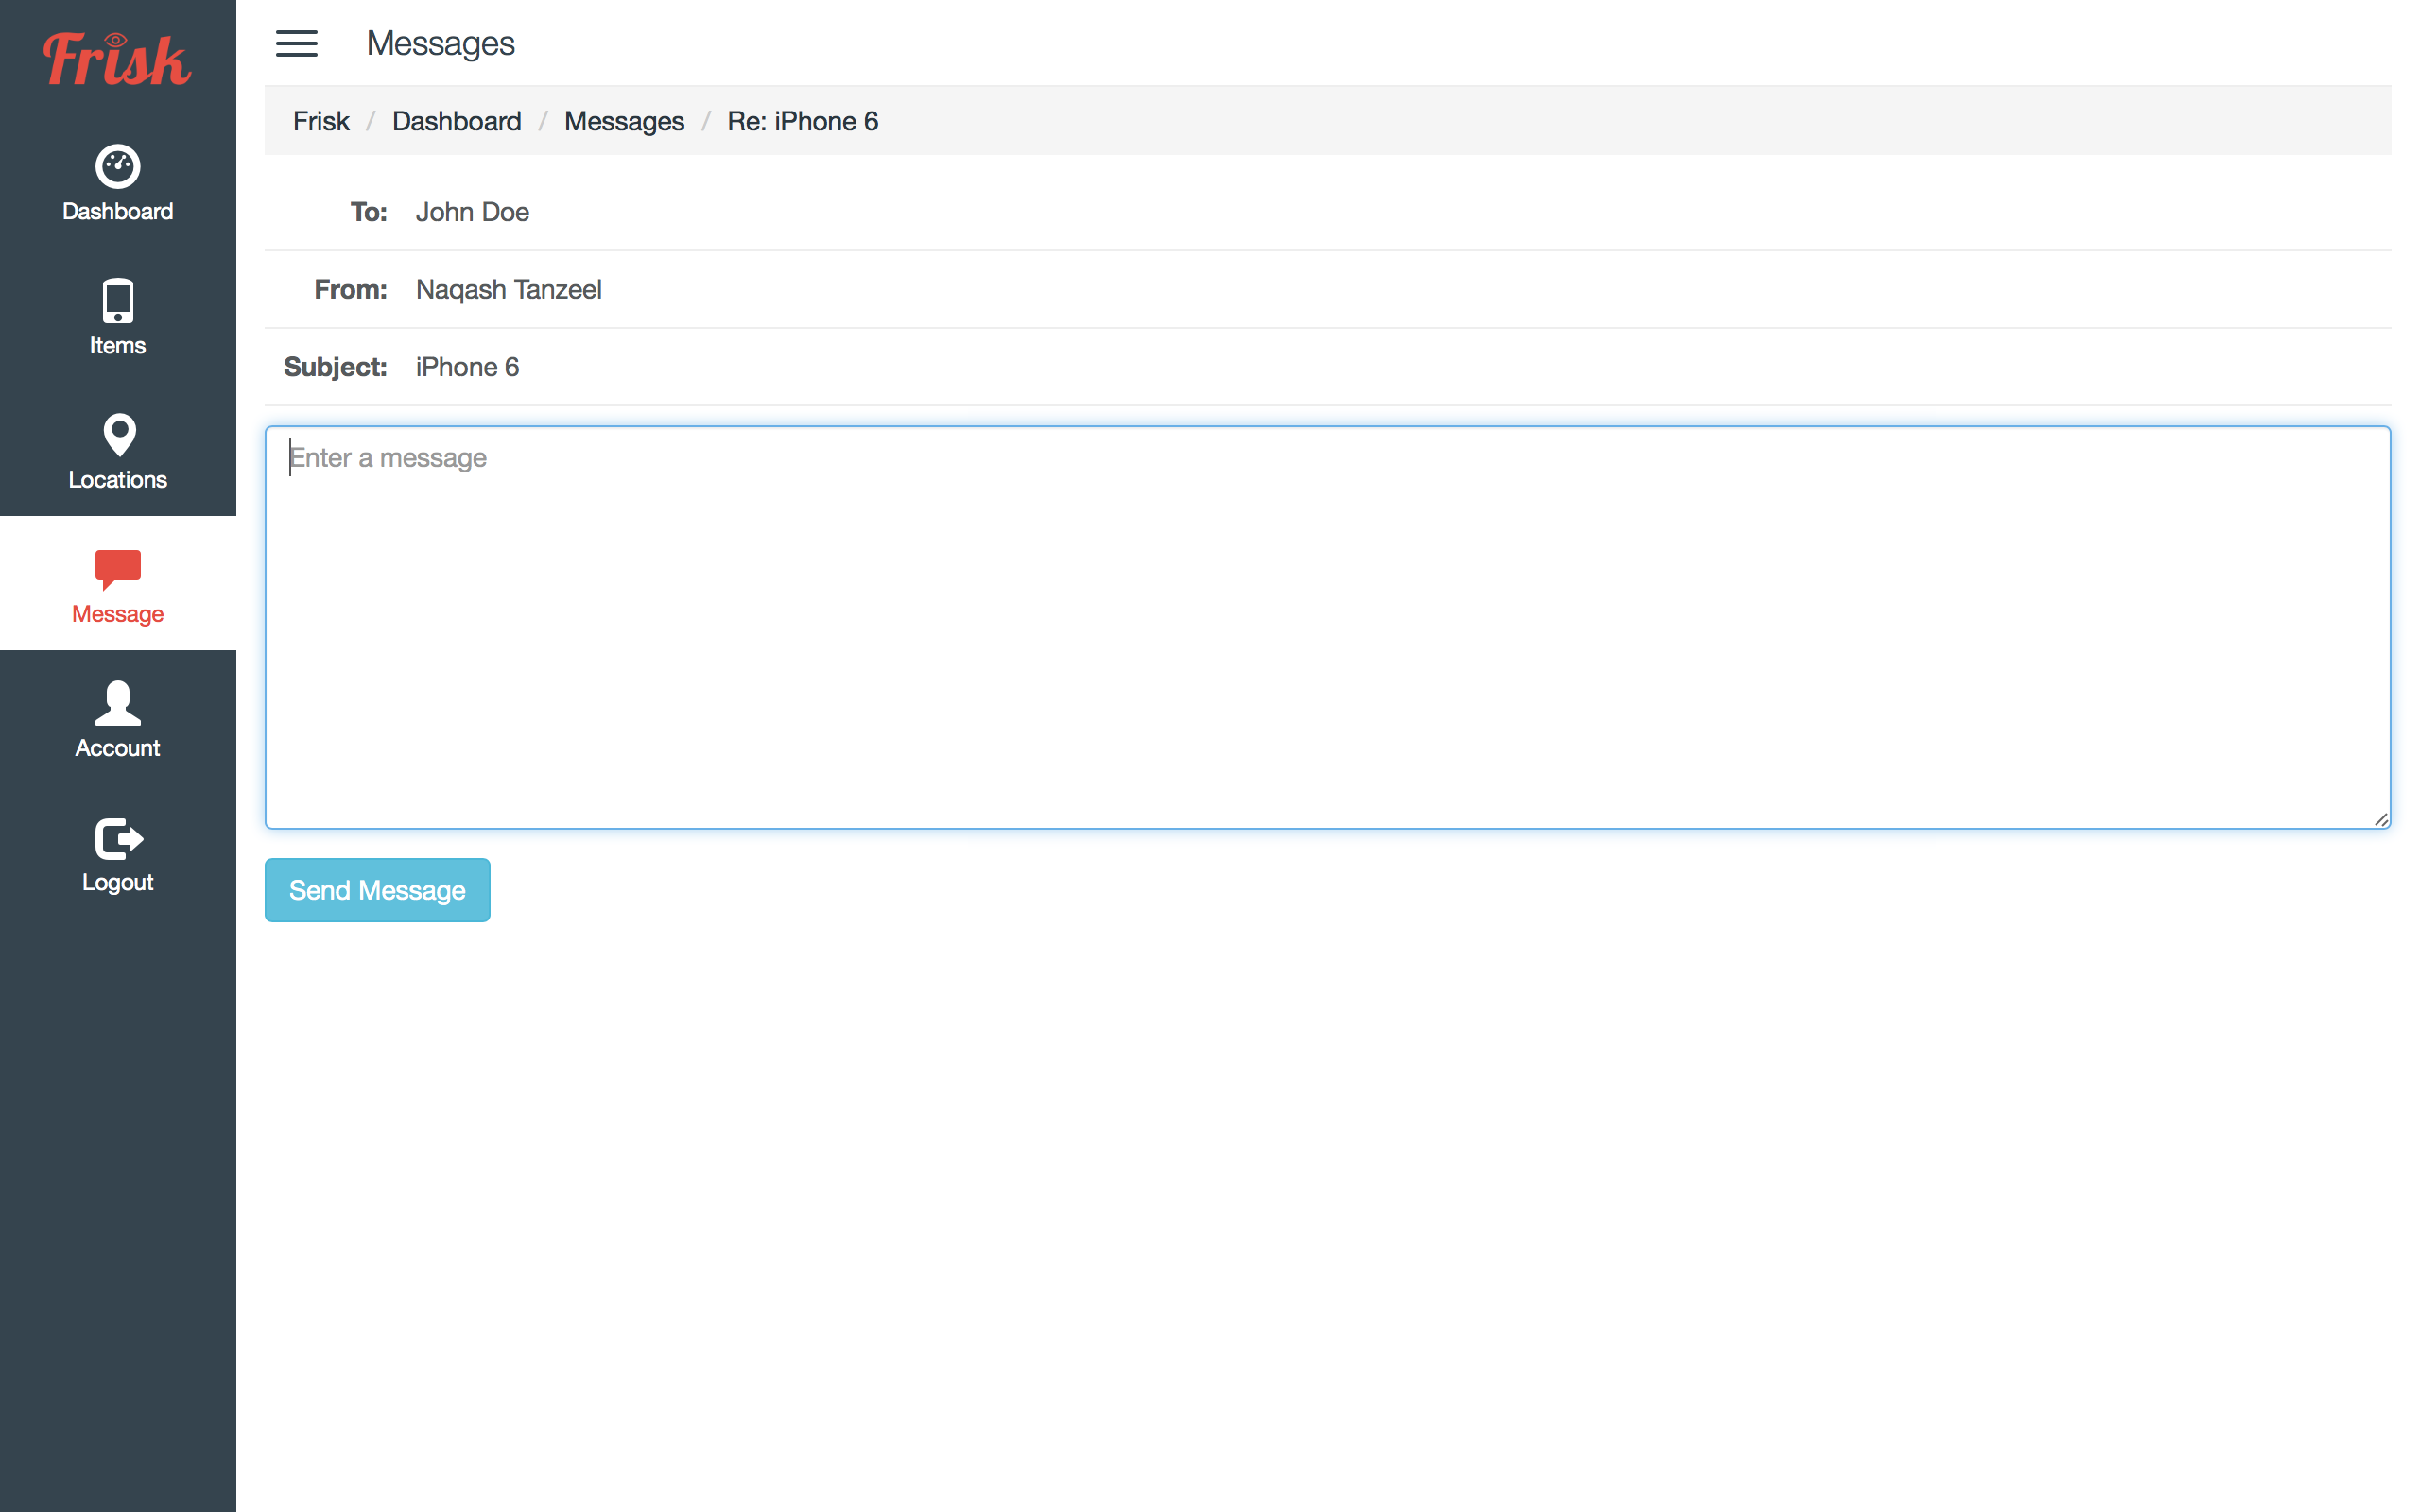
\includegraphics[width=1.0\textwidth]{images/Frisk/Dashboard_Create_Message}
	\caption{Frisk - Create or Reply to Message (Dashboard) } \label{fig:Dashboard_Create_Message}
\end{figure}

The create messages page will be a simple form which will allow the user to enter their message and nothing else (See figure \ref{fig:Dashboard_Create_Message}). The remaining details such as the recipient, subject and sender will be automatically filled in and will not be editable by the user. Viewing a message will display it in the exact same form as the form used to compose the message. The view form will provide a link in the page actions to reply to messages which will redirect the user to the create message form. This same form will be used for replying to a message. 

\subsection{Cross Platform Design - Responsiveness}
When designing the system it is important to keep in mind that a web application may be used across a range of devices with varying resolutions. This will strongly influence the design decisions made as certain features will be achievable on devices with lower resolutions whereas other features will make pages appear empty on larger resolution devices. Figure \ref{fig:Dashboard_Responsive} shows the locations page on different devices and shows how the page will adapt to these changing screen sized.

\begin{figure}[H]
	\centering
	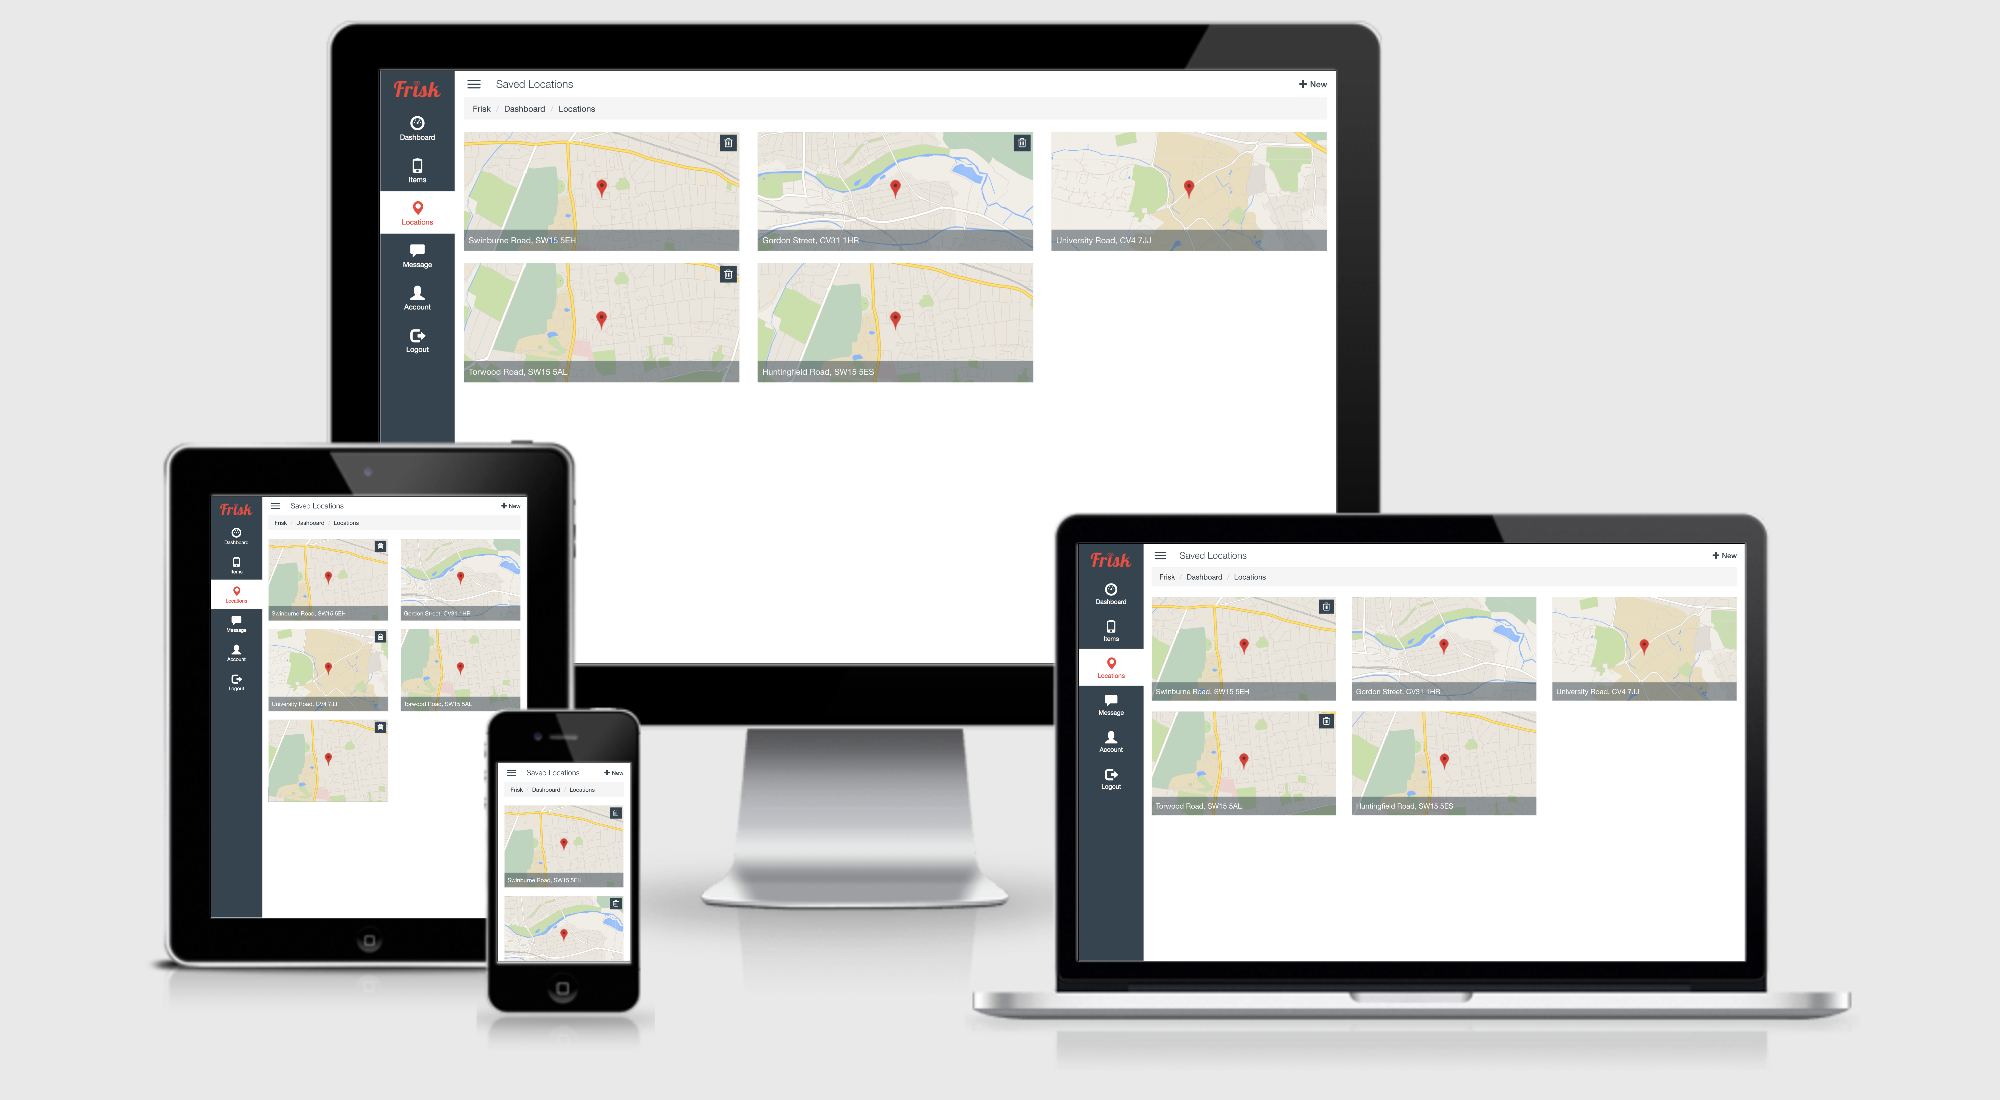
\includegraphics[width=1.0\textwidth]{images/Frisk/Responsive}
	\caption{Responsive Design - Locations Page } \label{fig:Dashboard_Responsive}
\end{figure}

The system must be easily usable regardless of the device the system is being viewed on, as long as a modern browser is used. The navigation will be hidden on devices with smaller screen to make more room for content on the page. In addition to this, content will be resized based on the size of the screen so that it is clearer and can be read easily without having to pan in and out.
\newpage